%%%%%%%%%%%%%%%%%%%%%%%%%%%%%%%%%%%%%%%%%%%%%%%

\newif\ifdigital

% Digital version of the PDF
\digitaltrue
% printed version of the PDF
% \digitalfalse 

% 2 side format
\ifdigital
  \documentclass[epsfig,a4paper,11pt,titlepage,twoside,openany]{book}
\else
  \documentclass[epsfig,a4paper,11pt,titlepage,twoside,openodd]{book}
\fi
\usepackage{epsfig}
\usepackage{plain}
\usepackage{setspace}
\usepackage{hyperref}
\usepackage{cleveref}
\usepackage{siunitx}
\usepackage{geometry} % layout setting

\ifdigital
  % DIGITAL: Equal left (inner) and right (outer) margins
  \geometry{
    paperheight=29.7cm,
    paperwidth=21cm,
    total={17cm,25.7cm}, % Automatically calculates symmetric margins (2cm each side)
    top=2cm,
    bottom=2cm
  }
\else
  % PRINT: Asymmetric margins for binding (inner=2.5cm, outer=1.5cm)
  \geometry{
    paperheight=29.7cm,
    paperwidth=21cm,
    inner=2.5cm,
    outer=1.5cm,
    top=2cm,
    bottom=2cm
  }
\fi

\usepackage{titlesec} % custom setup title of chanpter
% \usepackage{newtxtext,newtxmath} % times new roman


%%%%%%%%%%%%%%
% support for accented letters
%
%\usepackage[latin1]{inputenc} % Windows;
\usepackage[utf8x]{inputenc} % Linux (unicode package is required);
%\usepackage[applemac]{inputenc} % Mac.

\singlespacing

% italian language
%\usepackage[italian]{babel}

\begin{document}

  % no page number
  \pagenumbering{gobble} 
  \input{front}

  \clearpage
 
%%%%%%%%%%%%%%%%%%%%%%%%%%%%%%%%%%%%%%%%%%%%%%%%%%%%%%%%%%%%%%%%%%%%%%%%%%
%%%%%%%%%%%%%%%%%%%%%%%%%%%%%%%%%%%%%%%%%%%%%%%%%%%%%%%%%%%%%%%%%%%%%%%%%%
%% Note
%%%%%%%%%%%%%%%%%%%%%%%%%%%%%%%%%%%%%%%%%%%%%%%%%%%%%%%%%%%%%%%%%%%%%%%%%%
%% Thanks/ Acknowledgements section is optional
%%%%%%%%%%%%%%%%%%%%%%%%%%%%%%%%%%%%%%%%%%%%%%%%%%%%%%%%%%%%%%%%%%%%%%%%%%
%%%%%%%%%%%%%%%%%%%%%%%%%%%%%%%%%%%%%%%%%%%%%%%%%%%%%%%%%%%%%%%%%%%%%%%%%%
  % \input{acknowledgements}
  % \clearpage
  \pagestyle{plain} % no heading, footer with centered page number

  
  % page number with Arabic format
  \mainmatter

%%%%%%%%%%%%%%%%%%%%%%%%%%%%%%%%%%%%%%%%%%%%%%%%%%%%%%%%%%%%%%%%%%%%%%%%%%
%%%%%%%%%%%%%%%%%%%%%%%%%%%%%%%%%%%%%%%%%%%%%%%%%%%%%%%%%%%%%%%%%%%%%%%%%%
%% Note
%%%%%%%%%%%%%%%%%%%%%%%%%%%%%%%%%%%%%%%%%%%%%%%%%%%%%%%%%%%%%%%%%%%%%%%%%%
%% Length: approximately 70 pages.
%% These 70 pages include:
%%   table of contents
%%   abstract
%%   chapters
%% Exclude:
%%   title page
%%   acknowledgments
%%   attachments
%%%%%%%%%%%%%%%%%%%%%%%%%%%%%%%%%%%%%%%%%%%%%%%%%%%%%%%%%%%%%%%%%%%%%%%%%%
%%%%%%%%%%%%%%%%%%%%%%%%%%%%%%%%%%%%%%%%%%%%%%%%%%%%%%%%%%%%%%%%%%%%%%%%%%

    % index
    \tableofcontents
    \clearpage
    
    
          
    % group to define space between chapters
    \begingroup
      % no page break between chapters
      % override clear page commands
      % \renewcommand{\cleardoublepage}{} 
      % \renewcommand{\clearpage}{} 
      % override format of title chapter
      % from
      %   Chapter X
      %   Title
      % to
      %   X   Title
      
      \titleformat{\chapter}{\normalfont\Huge\bfseries}{\thechapter}{1em}{}
        

      \titlespacing*{\chapter}{0pt}{0.59in}{0.02in}
      \titlespacing*{\section}{0pt}{0.20in}{0.02in}
      \titlespacing*{\subsection}{0pt}{0.10in}{0.02in}
      
      % summary / abstract
      \chapter*{Abstract} % no number
\label{abtract}

\addcontentsline{toc}{chapter}{Abstract} % add to index


The additive manufacturing technology (i.e. 3D printing) has gained substantial popularity in recent years,
both in an industrial settings (where technologies such as SLA and SLS dominate)
and in the consumer space (where FDM or Fusing Deposition Modelling printers are 
by far the most common option due to the lowe price).

The fast adoption of 3D printers mostly stem from the fact that
they allow to manufacture very complex shapes that would often be impossible to produce
using more traditional manufacturing techniques; However although they are very flexible
in the variety of producible shapes, 3D printers still can't construct any arbitrary
shape.

The biggest challenge that prevent an object to be printed in one piece
is gravity, and the impact it has on the layer segmentation procedure.
The vast majority of 3D printers works by constructing a particular object layer by layer,
where every layer is constructed by ``adding'' the material the desired places.
This of course create some issues when a large area need to be created
without having anything below (often referred to as ``overhangs''); 
In this case the layer cannot be deposited on top of anything,
meaning that most of the time it will foll down and cause a failed print.

The most common way to deal with overhangs is through the use of supports; 
A support is simply something that is printed together with a specific object,
but is only there to sustain a specific overhang region while it prints, and will
then be removed. The vast majority of support structures are not designed by hand,
but they rather automatically generated by specialized algorithms.

Supports are inherently wasteful, as they are often thrown away the moment that they are
detached from the printed object; This create a requirement on support structure optimization
algorithm, namely the objective of producing a support that minimizes the material combustion.
Some research in better support structure optimization algorithms already exist, both
in form of academic literature, and also as part of many popular open-source 3D printing softwares.

One key thing to understand however, is that support structures are not necessarily portable
across different 3D printing technologies,
Indeed some technologies (such as for example SLA, and to a minor extend SLS) exert minimal
forces to the object while it's being printed, meanwhile in DFM, the nozzle will always
put a bit of force onto the object is printing while it deposits the material. This means
that printing tall and skinny structures on a DFM printer often results in them bending
and ultimately causing the print to fail.
SLA and SLS 3D printing software often find themselves designing supports with
tall and skinny structures, as the thinker a support is, the least material ti consume.
FDM softwares however tend to construct structures that are a bit thicker, as support that are too
thin would result in them bending and or braking during printing.

A promising approach for reducing the material necessary to print a support is the use of 
Genetic Algorithms; Indeed this class of algorithms often excels at complex minimization
problems, where exact solutions are too complex to find. In literature we can find 
some examples of this algorithmic approach being applied for support generation,
however all the attempts were designed to work on SLS and SLA 3D printers,
while FDM is left unaddressed by the current literature.

Our work's aim is to fill the void in the literature by creating an genetic-algorithm
based support structure optimizer that is specifically designed with FDM 3D printers 
in mind. For achieving this objective we began by selecting a ``topology'' of the support 
structure. All of the previous literature had used tree-like structures with a fixed
size beam, this is fine for SLA and SLS but when testing this topology on a FDM printer
we found out that the tree wasn't stiff enough, and resulted in a failed print.
Meanwhile open source FDM 3D printing software is also using tree topologies,
but the thickness of the beams is greater at the bottom, making the entire structure
stable (but consuming more materials).
In our algorithm we decided to use a rigid frame topology (where unlike a tree
andy point can have multiple connections to the ground) with fixed-size beams,
as some early testing has shown promising results both in terms of stiffness and in terms
of material usage.
With the topology selected we then preceded designing an algorithm that was able to
optimize this topology based on a cost function.

One key component of the cost function is stiffness, as we want to prevent beam to bend and cause
a failure. however stiffness evaluation of a complex rigid frame is a time consuming process, and 
four our genetic algorithm to converge we need to run this evaluation process hundred of thousands
of times. For this reasons, instead of using traditional stiffness evaluation algorithms, we designed
our own faster alternative. Our algorithm is a monte-carlo approach, as we had to sacrifice a bit of 
accuracy in order to get the required speed. Our tests have shown that (for our specific use-case)
our algorithm is about 400 times faster, while only losing about 4\% of accuracy when compared
to exact methods.

The genetic algorithm was developed in a three stage step. This was done to reduce
the complexity of the problem, by separating it into three separate problems.
The three problems were: Selection of the contact points,
grouping of different areas together, and optimization of the support structures.
The final result is a reduction of approximately 43\% in the material usage
for supports when compared to the state of the art algorithm for FDM 3D printers.
The results where validated in the real world with real print tests, and all the 
models were printed successfully.

Our current approach have a few downsides including longer printing time
and a slightly worst print quality (which are caused by the design of 
the contact points, and we believe can be addressed in future work).
but is overall a substantial improvement over the current state of the art.
We believe that with a few refinements and ease of use improvement
our algorithm could save a measurable amount of plastic if 
it managed to get a wide adoption.




%%%%%%%%%%%%%%%%%%%%%%%%%%%%%%%%%%%%%%%%%%%%%%%%%%%%%%%%%%%%%%%%%%%%%%%%%%
%%%%%%%%%%%%%%%%%%%%%%%%%%%%%%%%%%%%%%%%%%%%%%%%%%%%%%%%%%%%%%%%%%%%%%%%%%
%% Note
%%%%%%%%%%%%%%%%%%%%%%%%%%%%%%%%%%%%%%%%%%%%%%%%%%%%%%%%%%%%%%%%%%%%%%%%%%
%% The first chapter of the final thesis must contain a summary of a 
%% maximum length of 3 pages, introducing the context and motivations,
%% resuming the problem faced by the student, the techniques used for the
%% investigation and the reached outcomes.
%% If the final thesis is developed in collaboration with other students,
%% the personal contribution of the student has to be underlined.
%%%%%%%%%%%%%%%%%%%%%%%%%%%%%%%%%%%%%%%%%%%%%%%%%%%%%%%%%%%%%%%%%%%%%%%%%%
%%%%%%%%%%%%%%%%%%%%%%%%%%%%%%%%%%%%%%%%%%%%%%%%%%%%%%%%%%%%%%%%%%%%%%%%%%      
      
      %%%%%%%%%%%%%%%%%%%%%%%%%%%%%%%%
      % chapters
      \chapter{Introduction}
\label{cha:introduction}

Additive manufacturing or AM (most commonly known as 3D printing) is the process of constructing a three-dimensional object
by means of depositing material (usually layer by layer) onto the object in order to achieve a desired shape.

The origins of this technology dates back to the 1980s, with the real ``3D Printer'' being created by Hideo Kodama, and described
in his paper ``Automatic method for fabricating a three‐dimensional plastic model with photo‐hardening polymer'' \cite{am_origins}.
During the 2000s 3D printing remained a fairly expensive process, with it's use being limited for prototyping inside of companies
that could afford it. A turning point in the history of the technology came in 2009, when the Fused Deposition Modeling (FDM) printing process 
patents expired, allowing many startups to ender the game.
In the following years, as the technology matured it become clear that 
AM could be used for more that prototyping, and some companies started leveraging its unique advantages in actual production lines.
One of the first industry to successfully integrate this technology in it's supply chain was the aviation sector,
where the ability to create higgle complex shapes is extraordinary helpful to reduce weight of various components.

While the technology was establishing a footprint in the manufacturing world, a separate innovation was happening on the side:
RepRap (Replicating Rapid Prototyper) \cite{reprap} was a project developed in the University of Bath, that aimed 
to develop an open source 3D printer that was cheap to produce.
The project was widely regarded as a success, and managed to build approximately 4500 machines in 2 and a half years.

In 2012 Prusa Research was founded and the company started selling it's famous i3 model \cref{fig:prusa_i3} (that was based on the RepRap project)
at a starting price of approximately €600. Since then consumer 3D printers have only become better and cheaper thanks to companies
such as Creatily, Elegoo and BambooLab.
\cite{print_pictures}



\begin{figure}[h]
    \centering
    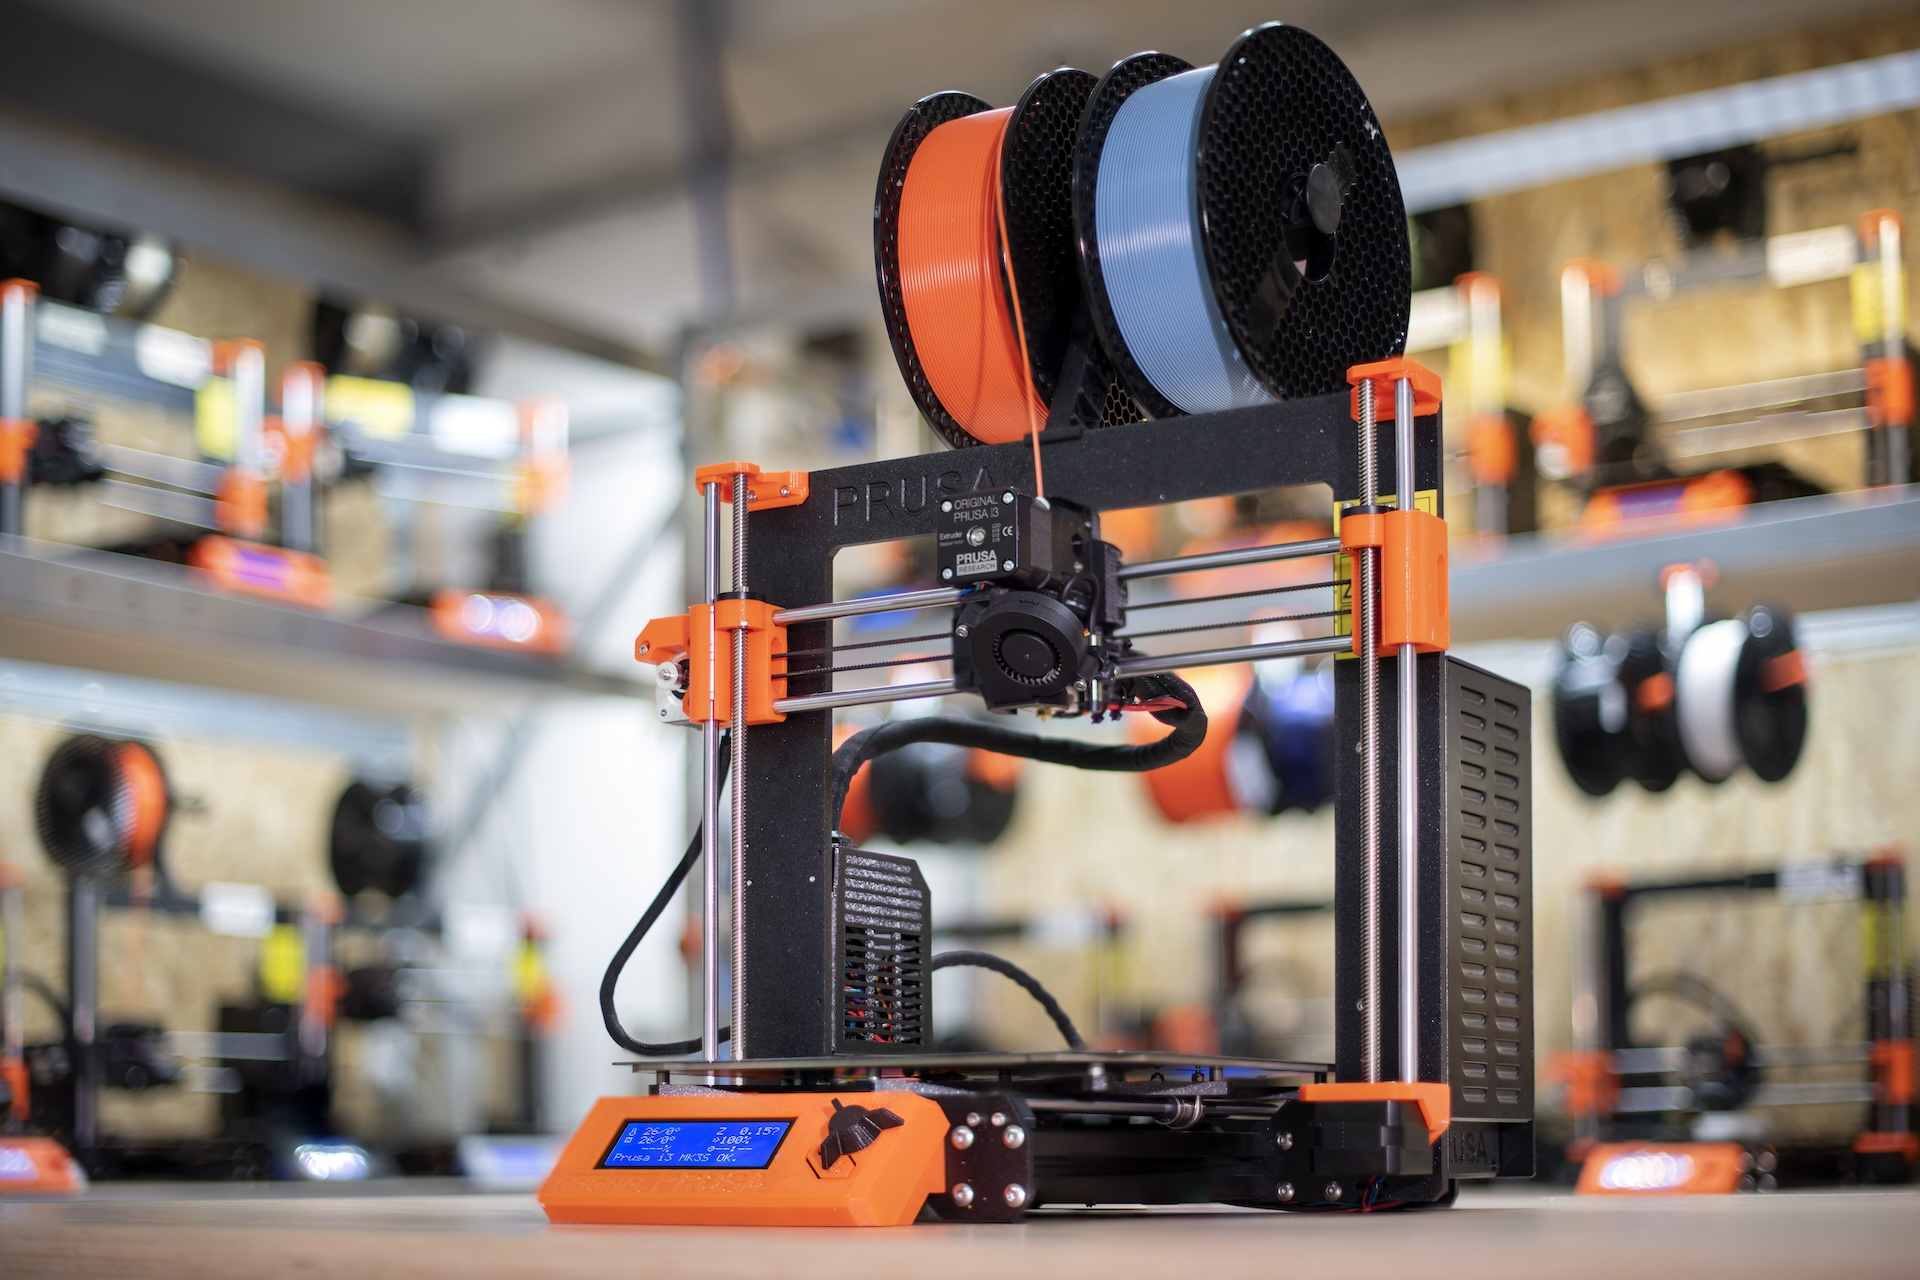
\includegraphics[width=0.33\textwidth]{images/prusa_i3.png}
    \caption{Original Prusa i3 Printer}
    \label{fig:prusa_i3}
\end{figure}


\section{3D printing technologies}

It is worth mentioning that the therm ``Additive manufacturing'' is a broad term that includes widely different techniques, each of them
has it's own strength and weaknesses. This section is not meant to be a comprehensive survey of all the 3D printing technologies, 
instead we will give a brief overview of the three most important techniques, and we will mention the advantages and disadvantage
of each of them, with a special focus on the forces that are applied on the printed object while it's being manufactured, which is
a factor that is particularly relevant for this thesis.

\noindent The techniques that we will explain in this section are:
\begin{itemize}
    \item Fused Deposition Modeling (FDM)
    \item Stereophotography (SLA)
    \item Selective Laser Sintering (SLS)
\end{itemize}
It is worth noting that an actual topology of 3D printing technologies is much more complicated than this simple list, however
the level of detail provided in this introduction is more than enough to understand the work presented in this thesis.

\subsection{Fused Deposition Modeling (FDM)}

Fused Deposition Modeling (FDM) is a technique that relies on a thermoplastic filament— that is fed by an extruder into a heated nozzle.
This nozzle melts the filament and moves through 3D space using a set of at least three motors.
To control this movement, a software program called a ``slicer'' converts a 3D model into a set of instructions known as ``gcode.''
These instructions are then processed by the printer's controller, guiding the nozzle to deposit the material layer by layer 
until the final object is created.


\begin{figure}[h]
    \centering
    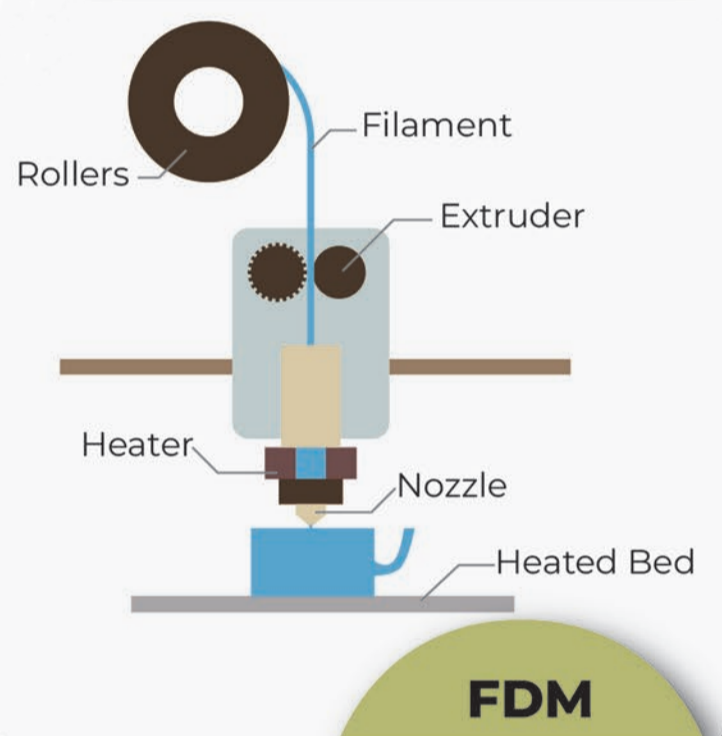
\includegraphics[width=0.33\textwidth]{images/fdm.png}
    % \caption{FDM technology overview (source: Martins 2023 \cite{print_pictures})}
    \caption[FDM technology overview.]{FDM technology overview (source: Martins 2023 \cite{print_pictures})}
    \label{fig:fdm}
\end{figure}

FDM is currently the most common 3D printing techniques for ``hobbyist'', as it's the cheapest option available, 
have good print dimensions (with most 3D printer having a build volume of 256x256x256mm).
Another advantage of FDM printing is the wide variety of usable materials, some of them (like PLA) are cheap,
and easy to print, others like ABS are more durable. Then there are a series of exotic material that offer
specific features, for example TPU is a material that is flexible and allow to print soft surfaces, while PVA
is a material solvable in water and is often used to print supports that can be removed simply by submerging
the printed object in water.
Another feature that is exclusive to FDM printer is the ability to print with multiple materials,
this is done with either a mechanism that automatically switch the filament used, or with printers that
have multiple nozzles.



\subsection{Stereophotography (SLA)}

\begin{figure}[h]
    \centering
    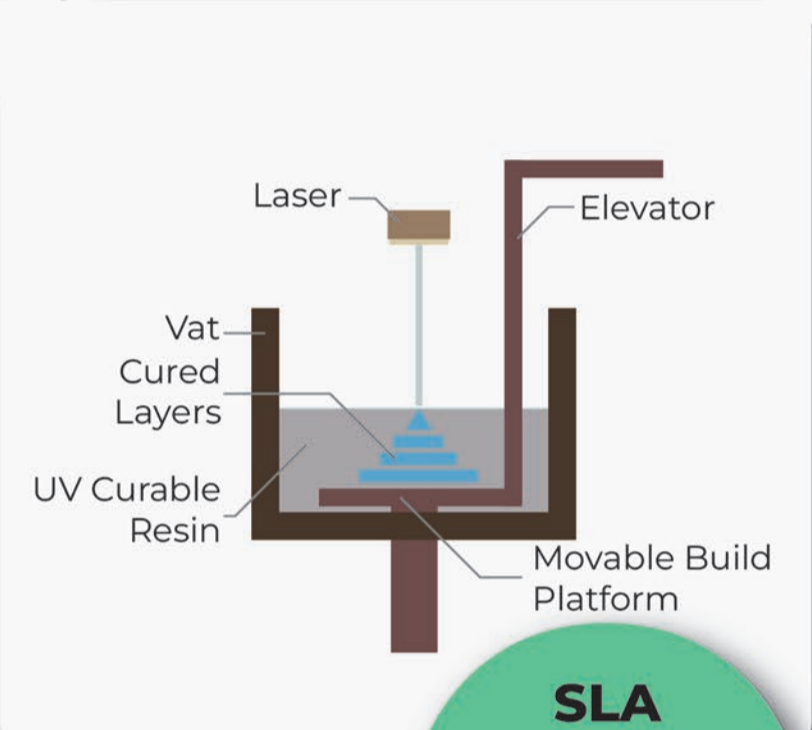
\includegraphics[width=0.33\textwidth]{images/sla.png}
    \caption{SLA technology overview (source: Martins 2023 \cite{print_pictures})}
    \label{fig:sla}
\end{figure}
Fused Deposition Modeling (or FDM for short)


\subsection{Selective Laser Sintering (SLS)}

\begin{figure}[h]
    \centering
    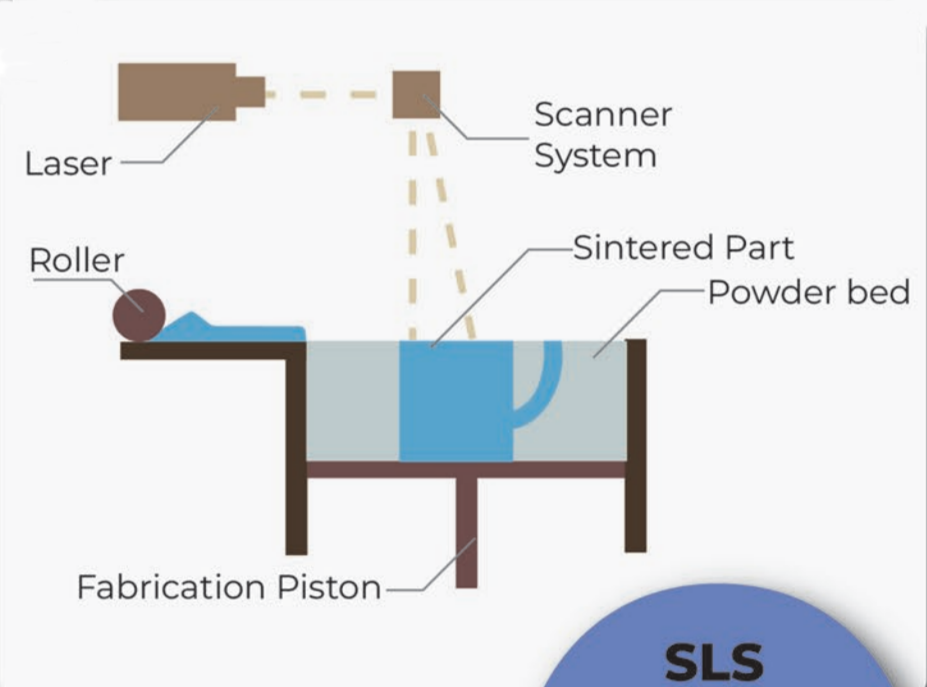
\includegraphics[width=0.33\textwidth]{images/sls.png}
    \caption{SLS technology overview (source: Martins 2023 \cite{print_pictures})}
    \label{fig:sla}
\end{figure}
Fused Deposition Modeling (or FDM for short)




      \chapter{Previous Literature}
\label{cha:prev_literature}

The idea to reduce the amount of plastic wasted on supports with the use of better
generation algorithms is certainly not a new one, and there is a lot of ongoing
research on the topic. However most of the research is conducted by companies in 
the space, and by open source developers, with only a fraction of it ending up
in academic research. For this reason this section is divided into two parts,
in the first one we will give an overview of the papers that are adjacent
to this thesis (namely papers that apply genetic algorithms to ghe generation
of supports); In the second section we will take a look at the industry standard
algorithms for support generation.
The reason why this thesis considered solution coming from open source software, and 
from the industry, rather than limiting to the academic research that was available is simple:
The academic research on the topic is a quite sparse (only two papers were found at the time of writing).
Furthermore as we will discuss in section \ref{sec:limitations}, the approach taken by the authors is not
really suitable for FDM 3D printing, and focuses more on SLA. Moreover none of the related works in section \ref{sec:acc_lit}
have made the code available, and this make the process of comparison impossible.
For those reasons the choice was made to include in this section some solution taken from open source
software, as they are the defacto standard used for support generation by 3D printing enthusiast
allow us to properly evaluate the proposed algorithm with some simple comparison.

\section{Academic Literature}
\label{sec:acc_lit}

\subsection[Genetic-algorithm based framework for lattice support structure optimization]{Genetic-algorithm based framework for lattice support structure optimization in additive manufacturing \cite{VAISSIER201911}}
\label{sec:paper_1}

This paper was the first one to apply genetic algorithms to support structure generation, and did so with a relatively
straightforward approach. They began by identify the overhanging (i.e. the zones that required supports)
(figure \ref{fig:paper_1} part 1), then they used a procedural algorithm to design a grid around the structure
(figure \ref{fig:paper_1} part 2). In the next step (figure \ref{fig:paper_1} part 3) a pre-processing was applied to remove 
from the structures the beams that could be excluded from the solution ``A priori''. Step 4 followed, where 
a genetic algorithm was used to prune the structure and remove further unnecessary beams, in this step the cost
function applied was a simple function of the volume of the supports (figure \ref{fig:paper_1} part 4). Finally a simple 
post-processing algorithm was applied, in order to further reduce he material used (figure \ref{fig:paper_1} part 5).
This is done with a series of simple steps such as for example connecting every two beams series with an individual
beam that will always be the same length or shorter as the sum of the other two.


\begin{figure}[h]
    \centering
    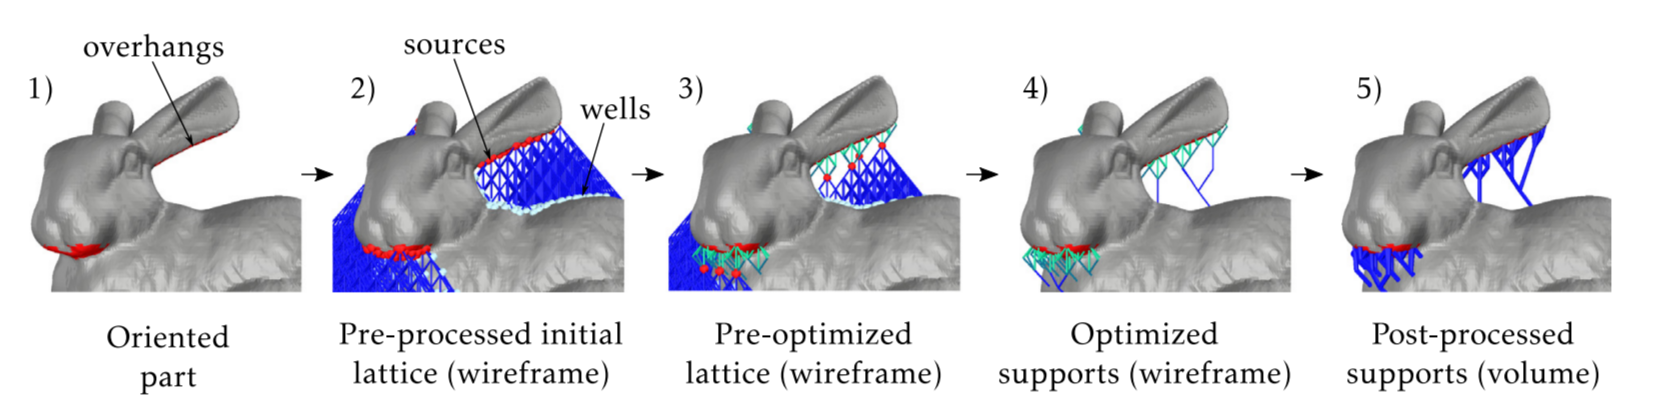
\includegraphics[width=0.95\textwidth]{images/paper1.png}
    \caption{Pipeline of paper \cite{VAISSIER201911}}
    \label{fig:paper_1}
\end{figure}

In the algorithm described above the grid was generated using a set of parameters (that were not subject to 
implicit optimization by the genetic algorithm) Those parameter were the height of a section, the distance
between the ``columns'', as well as the diameter of the beams, those parameters cam be seen in figure \ref{fig:paper_1_param}.
The authors emphasis how correctly selecting those parameters was essential for the quality of the results.


\begin{figure}[h]
    \centering
    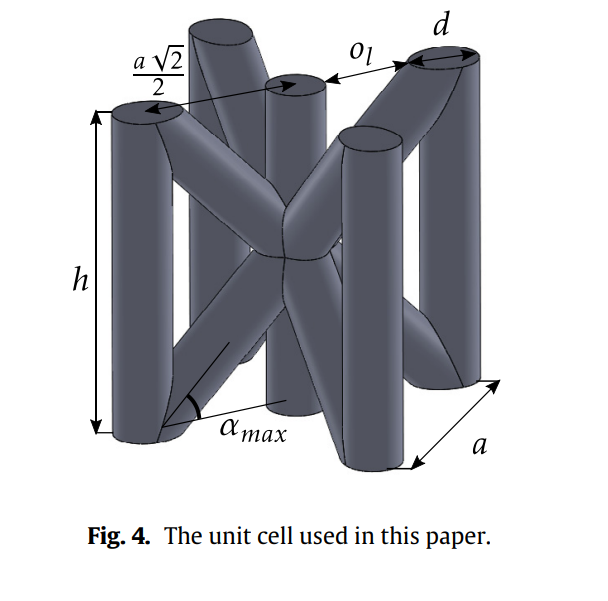
\includegraphics[width=0.4\textwidth]{images/paper1_params.png}
    \caption{Parameters used for structure (paper \cite{VAISSIER201911})}
    \label{fig:paper_1_param}
\end{figure}

The paper have also presented two different encoding structures to use in the optimization part (shown in figure \ref{fig:paper_1_encoding}).
The first strategy was called ``Activation Encoding'' where every beam of the graph was assigned
a boolean variable, where 0 meant that the node was removed, and 1 meant that the node was kept.
The first strategy was called ``Switch Node Encoding'' and essentially assumed every node could only be connected
to one of the possible downward directions, and the encoded variable simply selected one of the possible one.
The authors have shown how this approach drastically reduced the size of the search space, and made the optimizer's 
life a lot easier, thus making it faster and more accurate.


\begin{figure}[h]
    \centering
    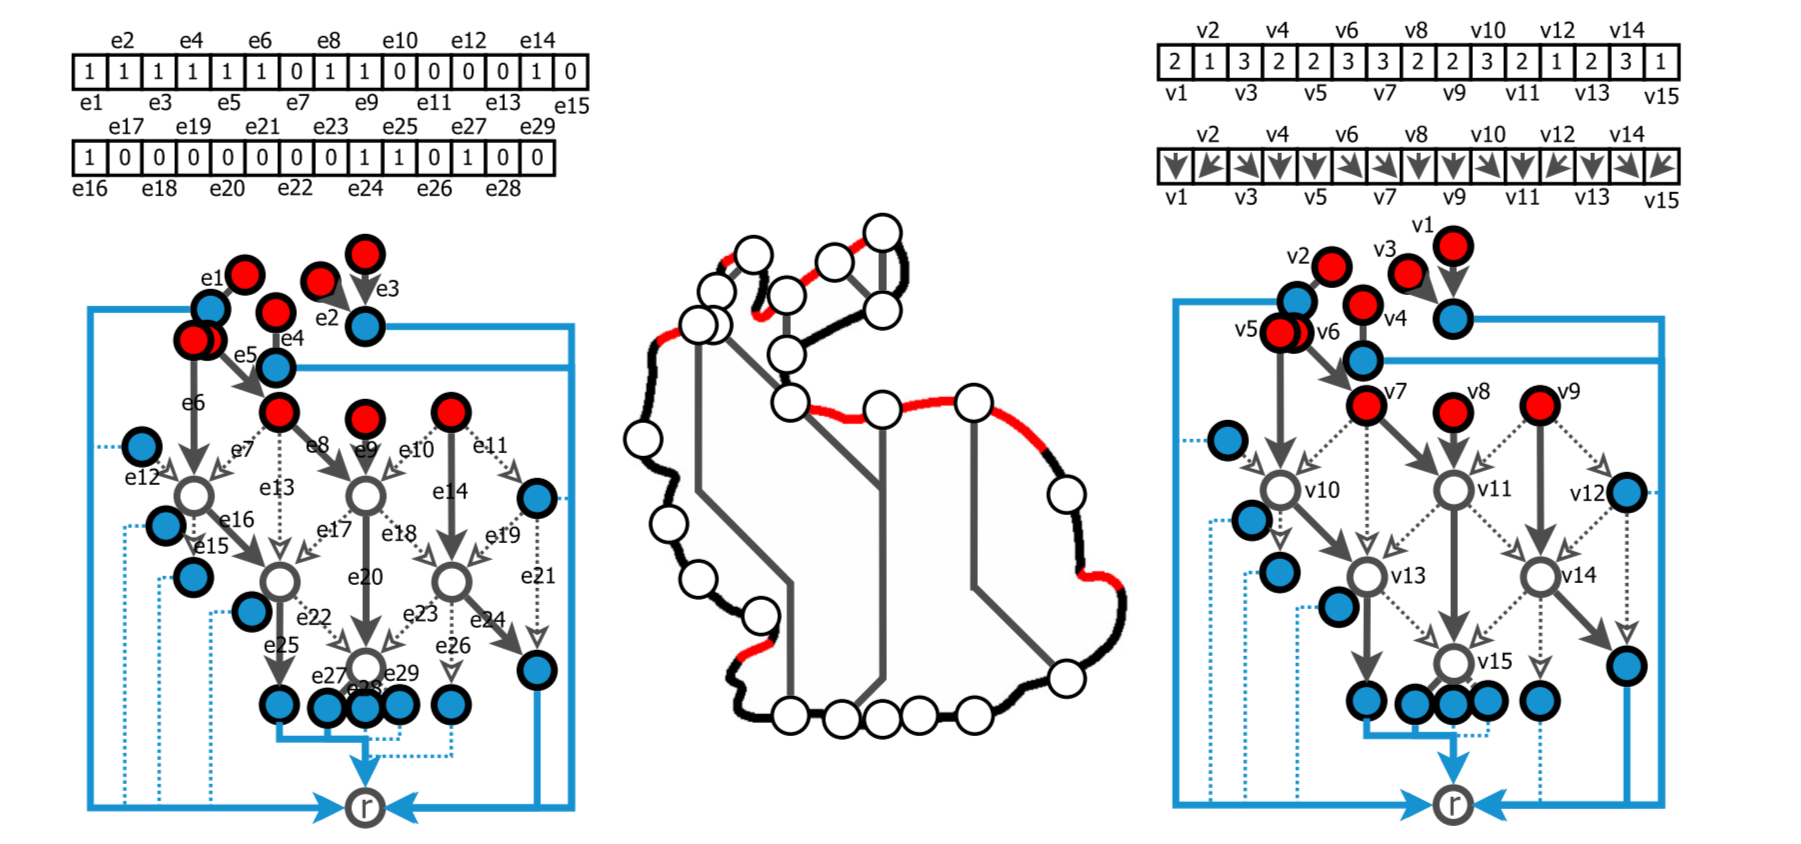
\includegraphics[width=0.95\textwidth]{images/paper1_encoding.png}
    \caption{The activation encoding (left), and switch node encoding (right) (paper \cite{VAISSIER201911})}
    \label{fig:paper_1_encoding}
\end{figure}

The paper concluded by testing the algorithm in a variety of meshes, and against a variety of support generation
algorithms selected from a academic papers, and a variety of industry standard tools.
They shown how their framework managed to reduce the use of material by 10-20\% compared to the the previous
best results.
The paper also shown one real world print made with their algorithm using a Laser Beam Melting (LBM) 3D printer
(which is a technology conceptually pretty similar to SLS). In conclusion this paper is quite relevant to the
work conducted in this thesis, as it's the first application of genetic algorithms for support structure optimization.
However their work was heavily focuses on LBM, and due to a set of factor that we will explain
in section \ref{sec:limitations} is not really applicable to FDM 3D printing.



\subsection[Bio-inspired generative design for support structure generation and optimization in Additive Manufacturing (AM)]{Bio-inspired generative design for support structure generation and optimization in Additive Manufacturing (AM) \cite{ZHANG2020117}}
\label{sec:paper_2}

This paper was also an developed with the idea to apply genetic algorithms to the problem of supports structure
optimization. The key novelty here was the introduction of a multi objective optimization program.
While in the previous paper \ref{sec:paper_1} the objective function was limited to minimizing the volume, in this
paper they focus on minimizing both the volume and the collisions \ref{fig:paper_2_collisions} among the support and the printed object.
Minimizing collisions is essential to ensure that the supports are easy to remove.
In order to optimize not only a single solution, but the set of pareto-optimal solution the authors used
the NSGA-II algorithms.

\begin{figure}[h]
    \centering
    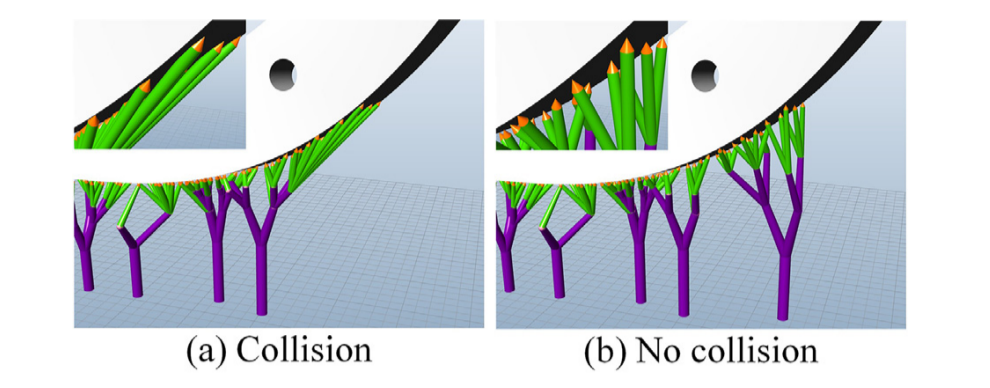
\includegraphics[width=0.5\textwidth]{images/paper_2_collisions.png}
    \caption{Collisions between the supports and the model (paper \cite{ZHANG2020117})}
    \label{fig:paper_2_collisions}
\end{figure}

One key novelty of this paper is the use of a dual stage optimization approach. They infact decided to
split the optimization into two separate problems. In the first one they find the critical structures, and they then
proceed to optimize the set of ``contact points'' (i.e. the position where the support structure will attach to the object)
This optimization problem is solved, and then they move on to the second stage, in which they used an L-System \ref{fig:paper_2_l_system}
who's parameters where optimized by genetic algorithms to optimize the structure of the trees.


\begin{figure}[h]
    \centering
    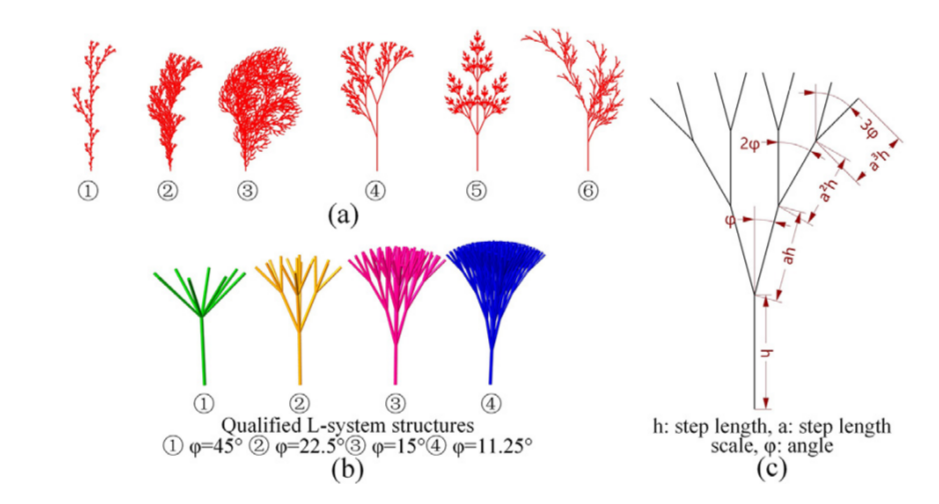
\includegraphics[width=0.5\textwidth]{images/paper_2_l_system.png}
    \caption{L-system used by zhang et. al. 2020 \cite{ZHANG2020117}}
    \label{fig:paper_2_l_system}
\end{figure}

Finally after a post-processing step that select one solution out of the evolved solution
a support structure is obtained. In the paper they tested the algorithm against
a collection of similar software and found that the reduction in use of material was approximately
40\%, Although it is wrath noting that they did only test prints of one object.
Nevertheless, the results are quite good, and can be seen in figure \ref{fig:paper_2_results}

\begin{figure}[h]
    \centering
    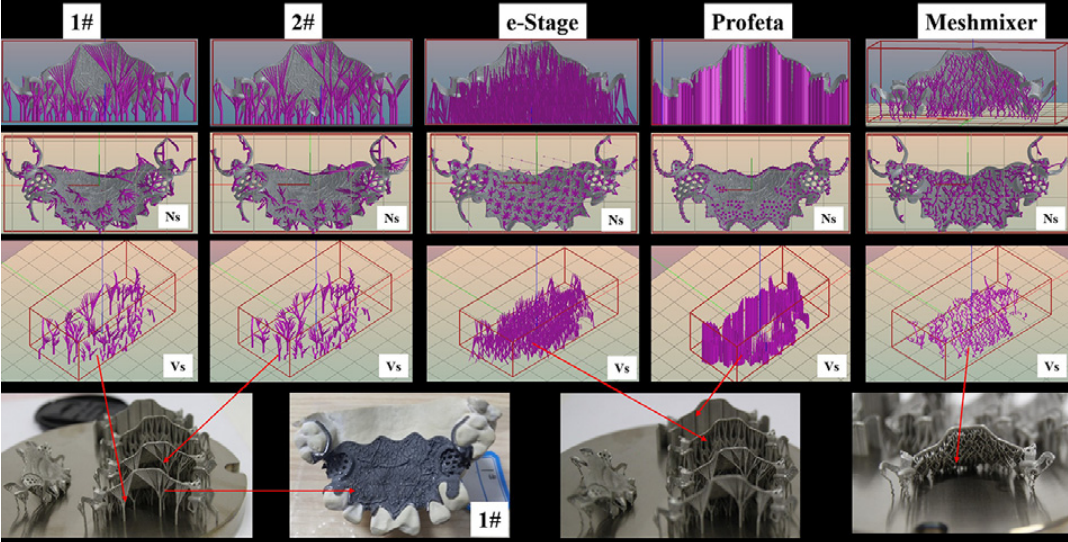
\includegraphics[width=0.5\textwidth]{images/paper_2_results.png}
    \caption{Result of zhang et. al. 2020 \cite{ZHANG2020117}}
    \label{fig:paper_2_results}
\end{figure}


\section{Industry Standard Solutions}


The Academic literature that was reviewed in the previous section is primarily geared towards
an industrial settings, and is therefore more focused on SLS  technologies (or similar), however
this thesis is more centered around the FDM technologies, and is therefore trying to solve a set 
of problems that is slightly different with respect to the papers that we just reviewed.
For this reason a second class of ``state of the art'' solutions is presented here.
This is a collection of support generation algorithms taken from the most used slicer for FDM printers
on the market.
The primary option to choose from here were OrcaSlicer \cite{orca_slicer} and Cura \cite{cura}.
However after a quick test it become clear that OrcaSlicer's support algorithms are superior
to cura in terms of material use, therefore they were selected as the key benchmark.

\subsection{``Normal Support'' (Orca slicer)}
\label{sec:normal_supports}

Normal supports are the one of the first example of auto-generated supports for 3D printing,
they are nothing special, as they are limited to a uniform wall create a zig-zag pattern in order
to reach the criticality region.
Compared to other techniques such as Tree support \ref{sec:tree_support}, those are considered a bit
wasteful.
Their inefficiency is simply given by the fact that the design is a straight wall that connect the critical
section at the top to the building plate as the bottom. Other more optimized algorithms try to merge multiple
critical areas together, in order to generate a single support that is narrower at the bottom, and brach out at the
top. This of course reduces the required materials.
Another key feature of modern support generation algorithms, that this algorithm doesn't have is a clean way
to handle supports that are ``multi layer'' (defined as a critical area that instead of having a direct line of sight
to the build plate have another part of the printed object that block the direct path from the critical area to the floor).
e can see this clearly in figure \ref{fig:multi-layer-support},
where the the normal support algorithm, when faced with a ``multi layer'' support, simply create a structure that go
straight down, and that rest on the printed object. This is generally considered undesirable, as it create twice
as many contact point between the support and the object, thus making the support removal  process more complicated.


\begin{figure}[h]
    \centering
    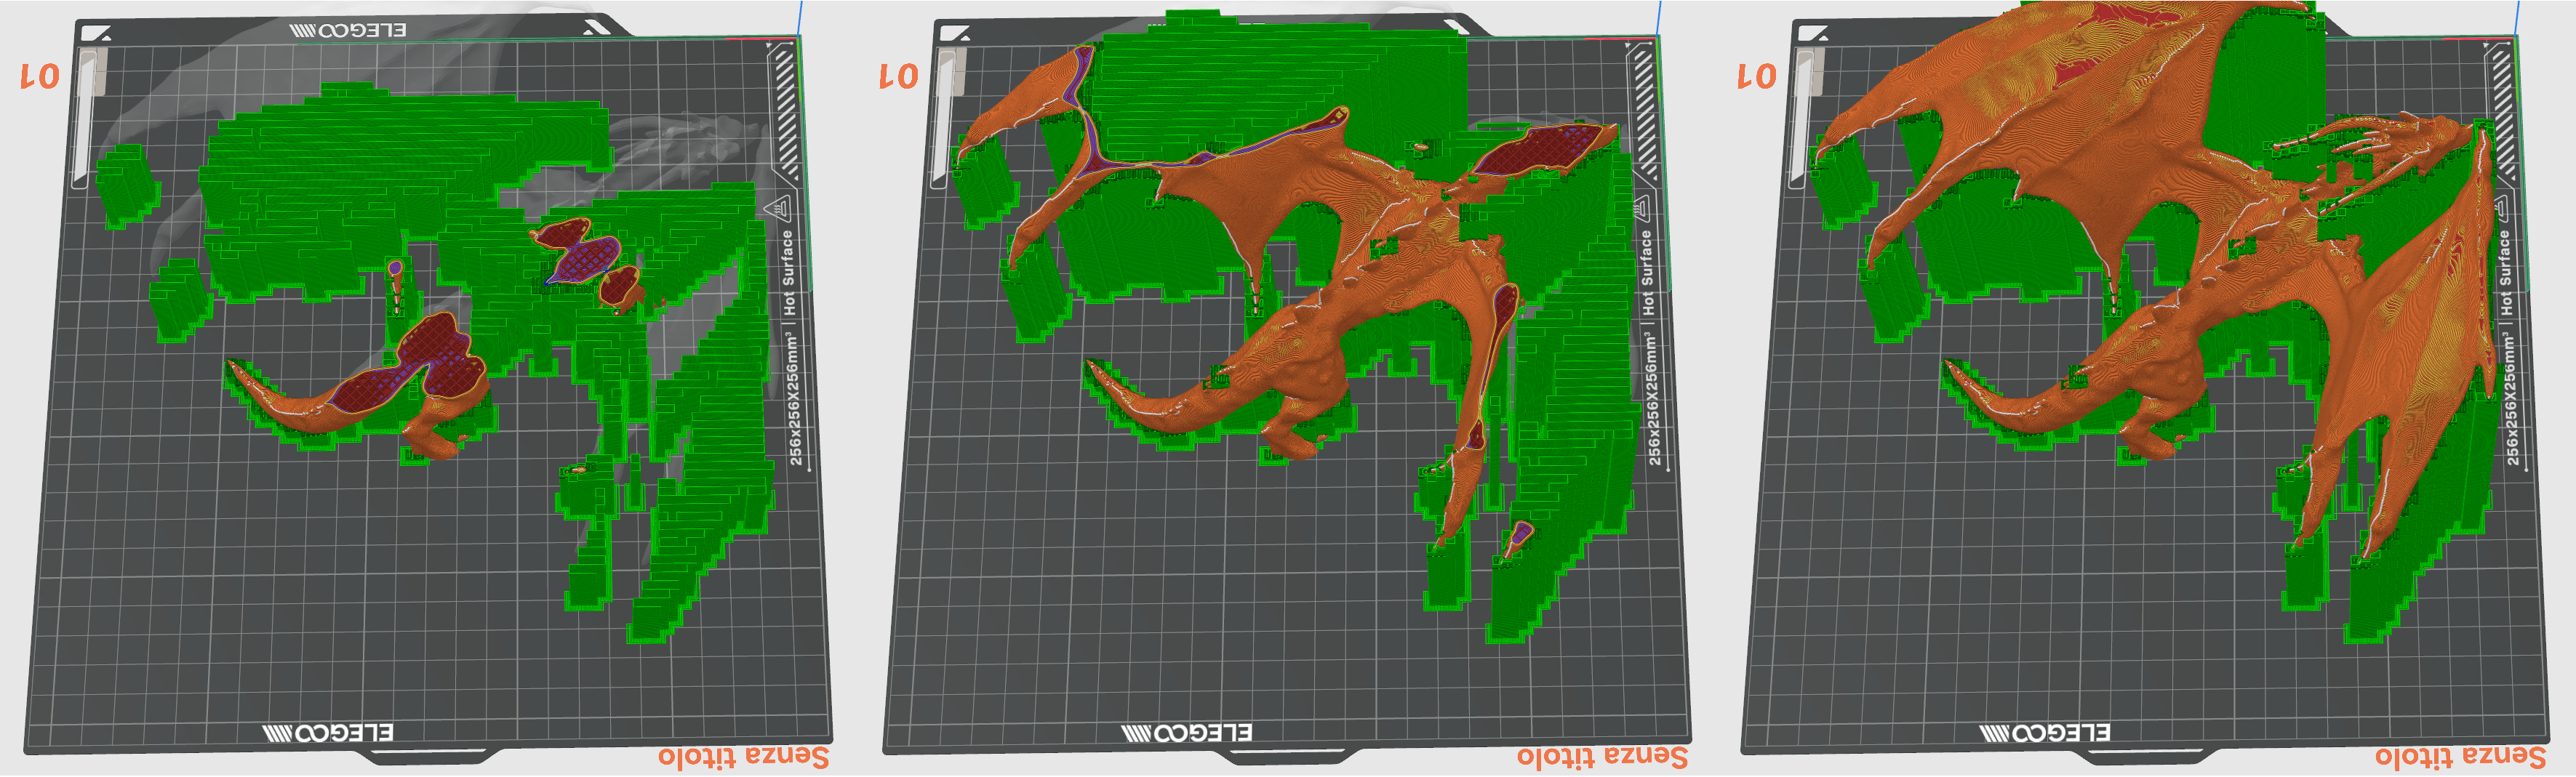
\includegraphics[width=1.0\textwidth]{images/normal_support.png}
    \caption{Normal supports (orca slicer)}
    \label{fig:normal_supports}
\end{figure}




\subsection{``Tree Supports'' (Orca slicer)}
\label{sec:tree_support}

Tree supports are the modern gold standard for lean support structure of FDM 3D printing.
They are a relatively new idea with the first version of their current form tracing back to 
an alpha release of Cura in late 2022 \cite{tree_supports}.
Every since then they have only improved, and they have become a beloved by the community.
Their design is incredibly simple and yet effective, critical regions that are close together
are merged into a single brach that move towards the plate, and gradually merge with other branches.
This is ensuring that the taller a critical area is, the more likely it is that it's support
will merge with others while moving towards the blate. This has proven very effective in reducing
the amount of material, as every two branches are merged we remove the need of having two
independent structures that go up to a certain height.

One key feature of tree support that should not be overlooked is the fact that the tree structures
are thicker at the bottom and they gradually get skinnier at the top. This is essential to ensure that
the supports can be printed correctly, as having supports that are too skinny at the bottom
would cause a z-wobble effect \ref{fig:wobble-test}, and thus leading to a failure.
It is also important to note that the tree get skinnier as it grows in order to save material, this can be done
due to the fact that when the nozzle is applying force by depositing the filament, the tree itself
is acting as a lever (with the fulcrum being the plate, and the force being applied where the nozzle is), 
and therefore the closer you are to are to the nozzle, the less advantageous the lever become, thus reducing
the amount of stiffness that the tree need to provide in order to not bend.



\begin{figure}[h]
    \centering
    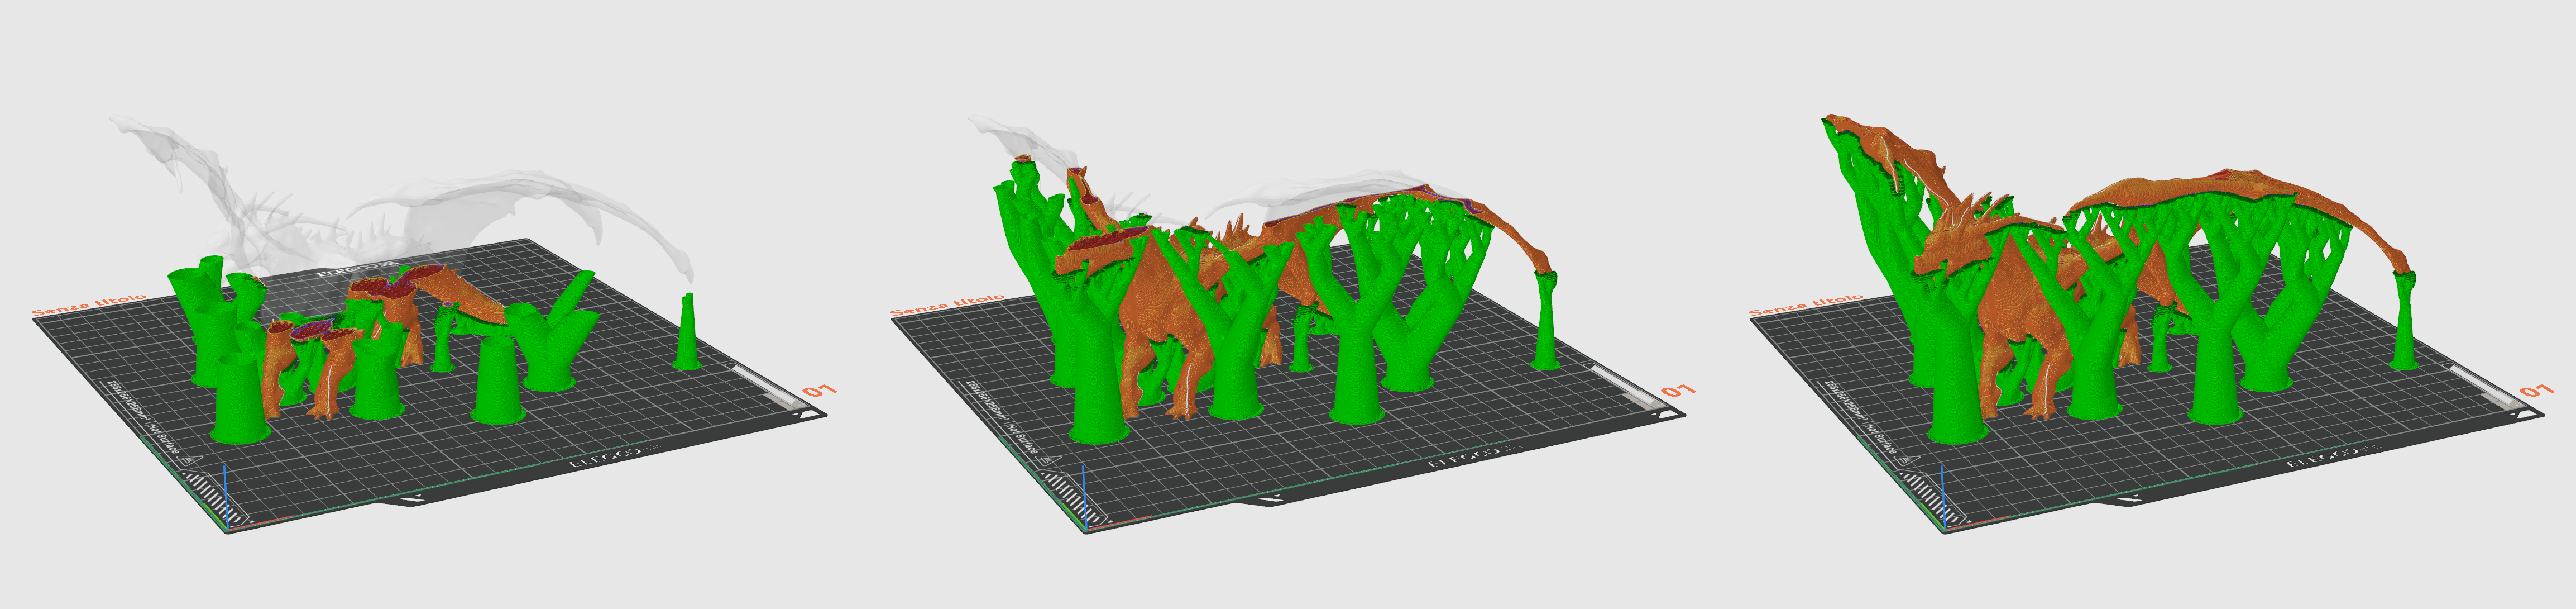
\includegraphics[width=1.0\textwidth]{images/tree_support.png}
    \caption{Tree supports (orca slicer)}
    \label{fig:tree_supports}
\end{figure}

One final feature of the tree supports is the way they handle ``multi layer supports'' (defined in \ref{sec:normal_supports})
As you can see in figure \ref{fig:multi-layer-support} when faced with this circumstance the algorithm try to find a diagonal
route that manage to support the critical area without intersecting with the printed object. This is feature is quite
liked by the community as it makes the supports easier to detach, even tho it increases slightly the amount of materials required 
for the supports.

\begin{figure}[h]
    \centering

    \begin{minipage}{0.48\textwidth}
        \centering
        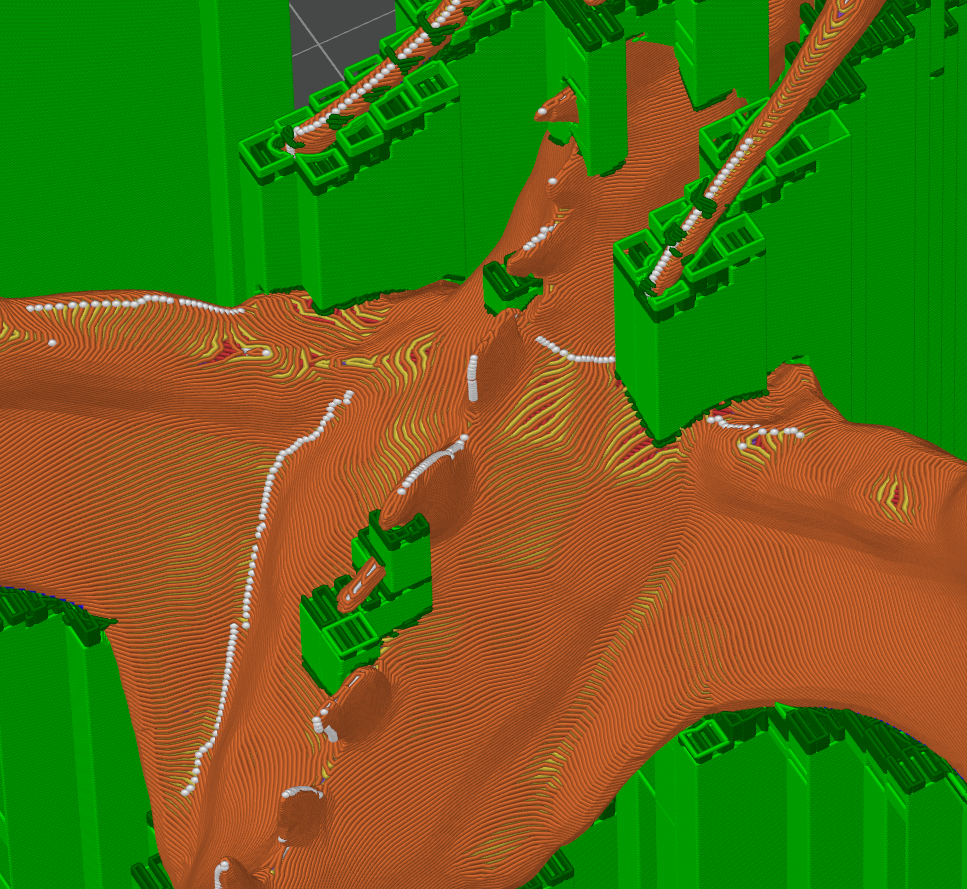
\includegraphics[width=0.9\textwidth]{images/munti_layer_supports_normal.png}
    \end{minipage}
    \hfill
    \begin{minipage}{0.48\textwidth}
        \centering
        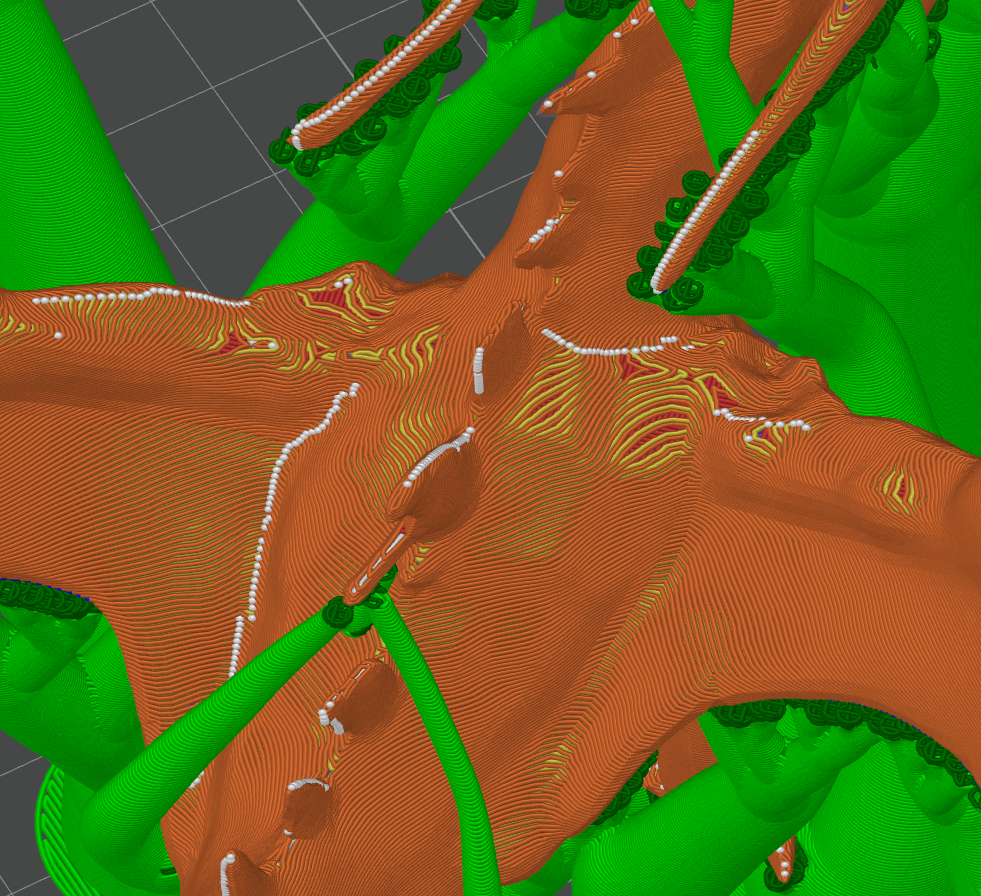
\includegraphics[width=0.9\textwidth]{images/multi_layer_supports_tree.png}
    \end{minipage}

    \caption{Handle of multi-layer supports (left: Normal supports, right: Tree supports)}
    \label{fig:multi-layer-support}
\end{figure}








      \chapter{Motivations}
\label{cha:motivations}

\section{Stated objective}

All the previous academic literature that we have locked at in section \ref{sec:acc_lit} is primarily
focused on industrial technologies such as SLS printing; This means that their work is not easily
applicable to other more consumer-oriented technologies (namely FDM), The reasons for this
are explained in section \ref{sec:limitations}, however 

\section{Limitation of previous work}
\label{sec:limitations}
\section{Choice of the support type}
\label{sec:sup_type}
\section{The missing part: Stiffness}
\label{sec:missing_part}
motivations



      \chapter{Monte Carlo Stiffness Evaluation}
      \chapter{Support Optimization Algorithm}
\label{cha:support_opt_alg}


\section{Pipeline Overview}
\label{sec:pipeline_overview}

The support structure optimization algorithm we are proposing is organized ino a pipeline
composed of 8 steps, of those the first and last are simple I/O steps (namely Importing and Exporting).
Then the steps two to four (Criticality Detection, Floating Regions Detection and Criticality Grouping)
are simple pre-processing steps that perform some operations in order to prepare data for the following
steps.
Finally steps five to seven (Contact Points Optimization, Contact Points Grouping and Support
Structure Optimization) are the real ``Optimization'' steps, that perform the optimization
of the actual support. This operation is performed in three stages, rather than a single optimization 
process for a more efficient computation, infact we can assume that the decision about where to place
contact points in the areas to support is (roughly) independent from the decision on how to build a
structure that reach those points, this allow to take the decision separately, and have two simpler
problems instead of one complex one. This approach is quite common in literature, infact it has
been used by Zhang et. al. \cite{ZHANG2020117} (the second paper we cited in the previous literature chapter).
The following lists show the steps of the pipeline in order, with a small description of what they do:

\begin{itemize}
    \item \textbf{Importing:} This step load the model and perform some simple re-meshing operations in order
    to reduce the amount of triangles in the mesh in order to obtain better performances.
    \item \textbf{Criticality Detection:} This step detect the critical regions (the points where the
    surface is too steep, and a support is required)
    \item \textbf{Floating Regions Detection:} This step detect the ``Floating regions'' (areas
    of the model that, while being printed are completely detached from the plate for a period of time,
    as the connection is provided by layers above)
    \item \textbf{Criticality Grouping:} This step groups the critical areas detected in the step 2 into
    some areas that can be optimized separately (for more efficient computation)
    \item \textbf{Contact Points Optimization:} This step identify an optimal set of points where
    supports will be placed using a genetic algorithm and a cost function.
    \item \textbf{Contact Points Grouping:} This step group the contact points into areas based on proximity,
    this step is once again performed in order to optimize the different areas separately.
    The optimization is done using a Compositional Pattern Producing Network Based Genetic Algorithm.
    \item \textbf{Support Structure Optimization:} This step optimize the support structure using a genetic
    algorithm, this step is where the stiffness evaluation algorithm we developed previously is used.
    \item \textbf{Exporting:} In the final step we generate a support structure in a mesh based 
    on the optimized parameters, the structure is then exported in STL format.
\end{itemize}


\section{Importing}
\label{sec:importing}

The importing stage is conceptually very simple, A mesh of the object we want to generate support for
is loaded, and then re-meshed.
Re-meshing is a simple procedure that involve starting from a mesh that represent 
a specific object, and then apply a transformation with the aim of obtaining a different
mesh, that represent the same object, using a different set of triangles that satisfy 
some specific properties.
figure \ref{fig:remeshing} show three different meshes that represent the same object,
the first one is minimizing the number of triangles necessary to describe the object,
but is resulting in a set of triangles that is very irregular. The second image show
a re-meshing of the first one, where triangles are divided into smaller and smaller pieces
in order to obtain more regular triangles. The third one is also a re-meshing, but 
it is a more aggressive one, and results in smaller triangles.
For this project we have used an incremental remaster (an algorithm that perform 
recessing by means of progressively splitting and merging triangles in order to obtain
some desired properties). The specific implementation was taken from the popular
rust library ``baby-shark'' \cite{babyshark}.

\begin{figure}[h]
    \centering
    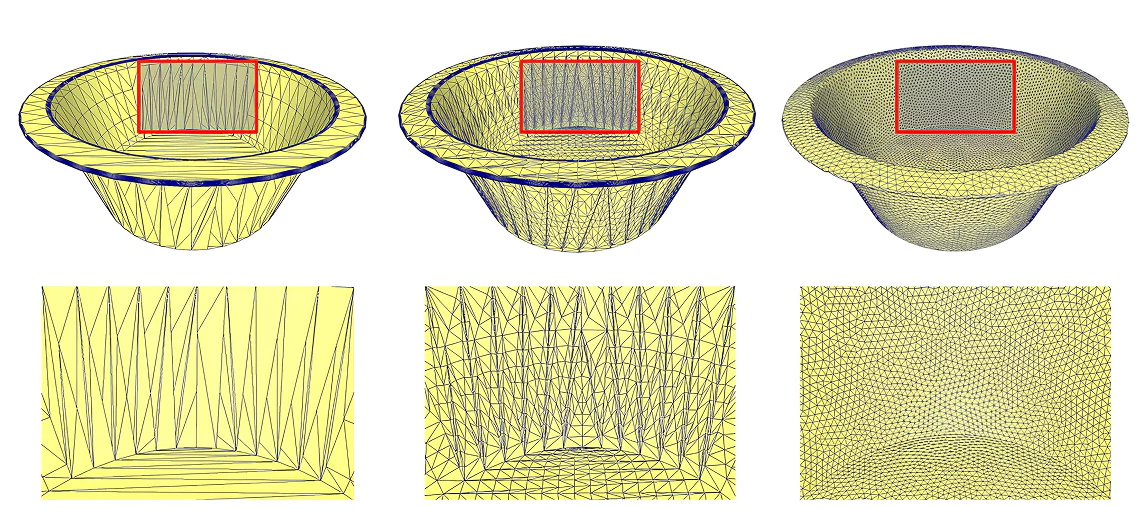
\includegraphics[width=0.5\textwidth]{images/remeshing.png}
    \caption{Example of a re-meshing operation (source: \cite{remeshing})}
    \label{fig:remeshing}
\end{figure}

There are two reasons why re-meshing is applied as part of the loading stage.
The first one is purely a performance reason, infact in order to generate support structure
we don't need an high definition mesh, instead a good approximation is enough. For this reason
the re-meshing process target an edge length in the range of 0.3 - 1.0 mm. this provide a sufficient
level of accuracy while also resulting in a manageable number of triangles, even for large meshes,
which helps the algorithm's performance.
The second reason why re-meshing is important has to do with the representation of the mesh
in the algorithm, infact the last step of the loading procedure is converting 
the mesh into a set graph, where every triangle is a node, and each node is connected
to three other neighbors (one for each side of the triangle.)
Generally speaking we would want all triangle to be as close to an equilateral as possible,
in such a way every connection inside the graph would have ruffly the same length; This
fact is a precondition necessary for the correct functioning of the next stages in the pipeline.
The re-meshing algorithm is therefore also used to ensure triangles have ruffly the same size,
and are ruffly equilateral.

\section{Criticality Detection}
\label{sec:crit_detection}

The first step in the generation of automatic support is of course knowing what zones must be supported.
Generally speaking the presence of a support or not is usually achieved with a simple check of the 
overhanging angle (as we already in the introduction \ref{sec:role_of_sup}).
One of the most basic technique for criticality detection is to simply take angle formed by the 
surface normal of a triangle, and a vector facing downward, and compare that to the threshold of what
is consider acceptable, in order to detect the critical areas.
Most 3D printing software use methods derived the one we just described with a few refinement
key refinements such as for example bridge detection, detection of areas that are ``floating''
etcetera. Our method also inspired by that basic idea, but is slightly different from the 
methods currently used in most commercial 3D printing software, as it's built with a different 
paradigm. Instead of simply detecting a simple boolean value that tell if a surface is critical
or not, our method aim to provide a cost function that, if minimized, reduces the amount of critical
areas there are in a specific model. The reason why this approach was chosen is straightforward, as 
is a simple consequence of the fact that we will need a cost function in order to apply a genetic-algorithms
based optimizer in the following steps.

Now that we explained the reasoning behind the creation of a custom solution for criticality detection
we can begin explaining our implementation. Algorithm \cref{alg:crit_det} show the pseudo-code of 
our implementation of a criticality detection procedure.
The key idea behind our solution is to assign to every node in the mesh graph a ``criticality''.
then the critical node are the one that have a criticality different than zero. This model has the benefit
that it can be easily transformed into a cost function by summing all the criticality score and 
weighting them by the area of the triangle they are associated to.
The second key idea that our solution brings to the table is the concept of ``criticality propagation''
This concept represent the fact that criticality is not an arbitrary value assigned to every single
triangle, regardless of the neighbors, instead the criticality is ``propagated'' from the bottom to the
top. This means that criticality increases every time the object have an overhanging angle that is too hig,
and decreases every time the criticality angle is too low. This is important because otherwise, a single
triangle inside the mesh with a sufficiently low overhanging angle would make an entire zone
less critical, or in the same way a single support could singlehandedly make a large critical area
no longer critical. Figure \ref{fig:critical_detect} show a mesh of a dragon, with the green areas
being the meshes with a criticality score of zero, while the red areas are the critical one.
In here we can see the effect that criticality propagation has on the structures.
in the bottom part of the dragon's wing we can see that the critical area is quite large,
even tho, the overhanging angle is quite small. We can get a sense on why propagation is important
by looking at figure \ref{fig:critical_detect_no_prop} and \ref{fig:critical_detect}.
In the former we see what are the critical regions if no propagation is applied, mean while in the second one
we see the same output, but propagation are applied. Te most notable difference is in the bottom part
of the dragon's wing, as we can see, in the version with no propagation there is a tiny critical area
in the tip of the wing, but as soon as the overhanging angle is small enough, the critical are disappear.
In contrast in the version that has propagation the criticality start at an high value in the top bottom
part of the wing, and require a bit of time for the score to reach zero, resulting in a much larger critical
region. This behavior is desirable, as is unreasonable to think that a single support in the tip of the wing
is enough to support the entire area, meaning that criticality propagation play a key role in detecting
more realistic critical regions when some part of the model are ``floating''.


\begin{figure}[h]
    \centering
    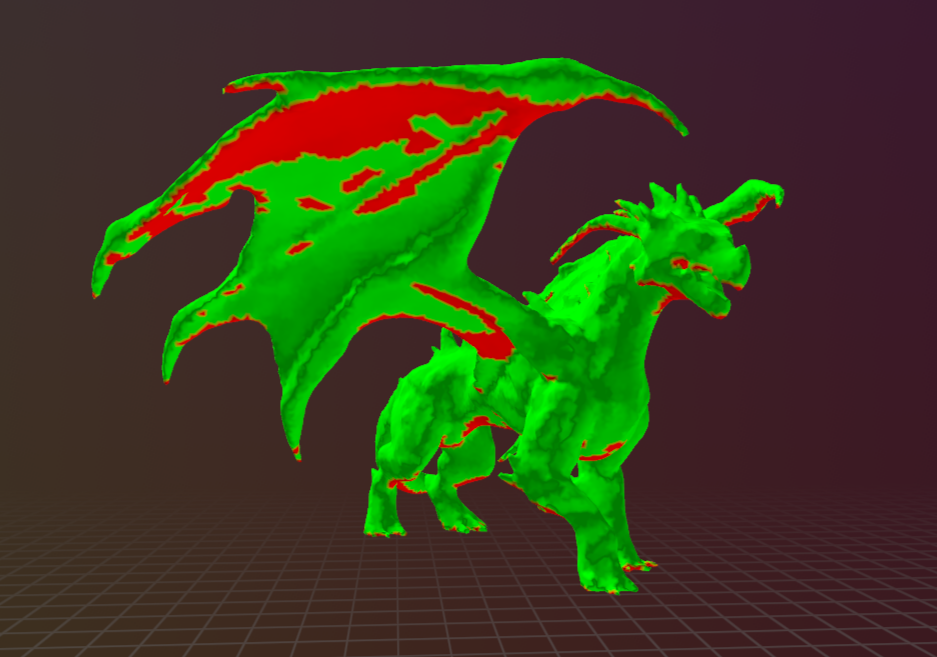
\includegraphics[width=0.5\textwidth]{images/critical_regions_w_no_prop.png}
    \caption{Critical regions detected by our algorithm, if no propagation is used}
    \label{fig:critical_detect_no_prop}
\end{figure}

\begin{figure}[h]
    \centering
    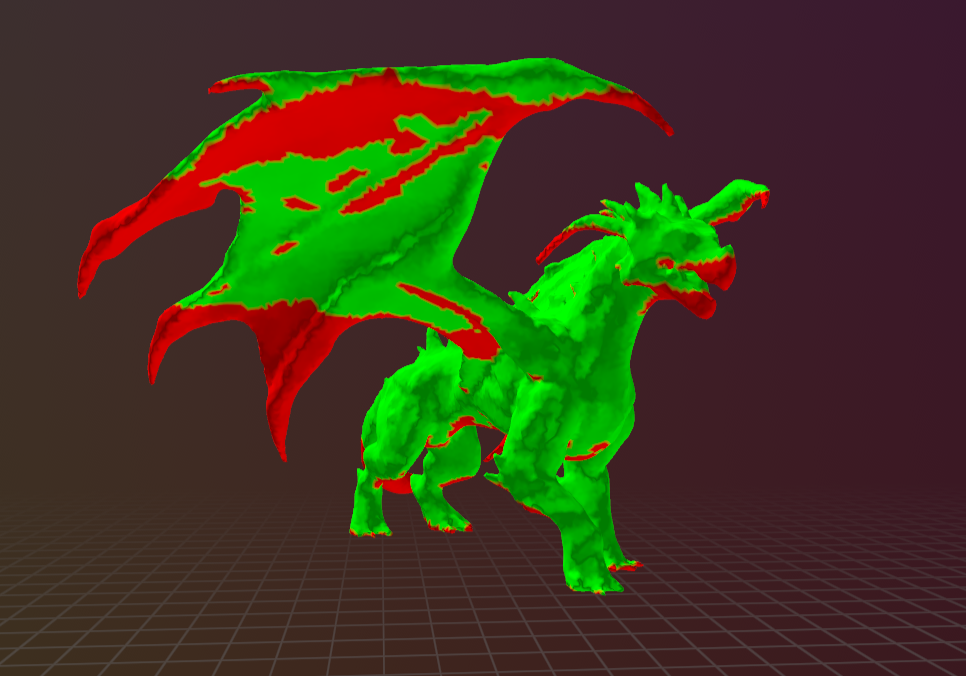
\includegraphics[width=0.5\textwidth]{images/critical_regions.png}
    \caption{Critical regions detected by our algorithm}
    \label{fig:critical_detect}
\end{figure}



\begin{algorithm}[H]
\caption{Criticality Detection}
\begin{algorithmic}[1]
    \Require $G$ Graph that represent the mesh
    \Ensure $C$ Dictionary that associate a cost for every node in the graph

    \Procedure{LayerOf}{$n$} \Comment{Calculate the layer of node $n$}
        \State \Return $\left\lfloor{\frac{\Call{Height}{n}}{L_{height}}}\right\rfloor$
    \EndProcedure

    \Statex

    \Procedure{PropagationCost}{$G, f, t$} \Comment{Calculate propacation factor of the link $f$(rom) $t$(o)}
        \State $\varphi \gets \Call{AngleBetween}{f, t}$ \Comment{We start from the angle between the two nodes}
        \State $\varphi' \gets \varphi - \varPhi_t$ \Comment{We compared to the threshold, as small gradients are OK}
        \State $\varphi'' \gets \Call{Clamp}{\varphi', \varPhi_{lb}, \varPhi_{ub}}$ \Comment{We clamp it, to avoid too high propagation factor}
        \State $d \gets \Call{Distance}{f, t}$ \Comment{Distance factor (long distance are more critical than short one)}
        \State \Return $K_{prop} \cdot d \cdot \varphi''$
    \EndProcedure

    \Statex

    \Procedure{CriticalityOf}{$G, n, \mathcal{M}$}
        \If {$\Call{Height}{n} = 0$} \Comment{Nodes to the ground are never critical}
            \State \Return 0
        \EndIf
        \State $c \gets $ CRITICALITY\_MAX \Comment{Initialize criticality at max value}
        \For{$a \in \Call{AdjacentNodes}{G, n$}} \Comment{Iterate over adjacent nodes}
            \If {$\Call{LayerOf} {a} <= \Call{LayerOf}{n} \land a \in M$}
                \State $c_a \gets M(a) + \Call{PropagationCost}{a, n}$
                \State $c \gets \Call{Min}{c, c_a}$
            \EndIf
        \EndFor
        \State \Return $\Call{Max}{c, 0}$ \Comment{Criticality is always greater of equal than zero}
    \EndProcedure

    \Statex

    \Procedure{PropagateInLayer}{$G, l, \mathcal{M}$}
        \State $ PriorityQueue \gets \emptyset$
        \For{$n$ in $l$} \Comment{Initialize the priority queue with the cost propageted by the laeyer below}
            \State $c \gets \Call{CriticalityOf}{G, n, \mathcal{M}}$
            \State $\Call{Push}{PriorityQueue, n, c}$
        \EndFor
        \While {$\lnot \Call{Empty}{PriorityQueue}$}
            \State $n, c = \Call{Pop}{PriorityQueue}$ \Comment{Extract node with the lowest criticality}
            \State $\mathcal{M}(n) \gets c$ \Comment{Mark the criticality in the memory}
            \For{$a$ in \Call{Adjacent}{$G, n$}} \Comment{Neighbors might now have lower criticality, update them}
                \State $c \gets \Call{CriticalityOf}{G, a, \mathcal{M}}$
                \State $\Call{TryUpdatePriority}{PriorityQueue, a, c}$
            \EndFor
        \EndWhile
        \State \Return $0$;
    \EndProcedure
    
    \Statex

    \Procedure{CriticalityDetection}{$G$}
        \State $C \gets \emptyset$

        \For{l in \Call{Layers}{$G$}}
            \State \Call{PropagateInLayer}{$G, l, C$} \Comment{Propaget the cost one layer at a time}
        \EndFor

        \State \Return $C$
    \EndProcedure
\label{alg:crit_det}
\end{algorithmic}
\end{algorithm}


\subsection{Algorithm Overview}
To explain \cref{alg:crit_det} we must start from the concept of layer.
Eery node in a graph is assigned to a layer (represented by an integer value),
the ``LayerOf'' function simply associate a node with is layer, and is simply using
the node's height as the discrimination factor;
The reason why layers are important is that the criticality can be propagated only from
elements of the same layer, or layer below, it can't go below a layer.
The function ``PropagationCost'' take as input two nodes, and calculate the cost that 
is propagated from one to the other in a specific direction, this means that if
node $A$ has criticality $c_a$ and the propagation cost from node $A$ to node $B$ is
$c_{ab}$ than the cost at node $B$ will be upper bounded by he value $c_a + c_{ab}$.
This is an upper bound because it can always be lower if node $B$ has another neighbor
from which it can propagate a lower cost.
It should be noted that this function can return a negative value, this is the case when 
the angle between the two nodes is below the threshold of the maximum overhanging angle, 
and therefore the criticality should decrease.
The function ``CriticalityOf'' is used to calculate the criticality of a node, starting
from nodes that are close to it; In the function we can see how if the node is close to the
ground the criticality is zero (this is obvious, as if a node is attached to the plate it does
not need any support), otherwise the criticality is initialized to the maximum possible value,
and then is reduced if a path is found to propagate a lower criticality value from a neighbor.
The neighbor in order to be eligible must be part of a layer that is the same or lower as the node
currently being evaluated.
Now that we have explained the few ``utility'' functions we can tackle the core part of the algorithm,
this is composed of the two functions ``PropagateInLayer'' and ``CriticalityDetection''.
the idea is that the criticality is propagated from bottom to top, then odes in the graph are organized
in layers, and layers are evaluated from the lowest to the hightest.
The process of evaluating a layer is essential a one pass of a Dijkstra algorithm, where nodes
are explored form the one with the lowest criticality value to the one with the highest.
This process ensure low time complexity while ensuring that every node has the correct criticality value.

\section{Floating Regions Detection}
\label{sec:floating_regions_detection}

Another important pre-processing step is the detection of ``Floating Regions''
As we mentioned in the introduction, a floating region is defined a part of the structure that that while being printed,
is not fully connected to the build plate if not for supports. For example
figure \ref{fig:floating_regions} show the floating regions of the mesh ``Dragon''
highlighted in different colors, while the plain mesh white.
In this section we will not explain why detecting floating regions is necessary,
as that topic will be extensively covered in one of the next sections (specifically \ref{sec:sup_struct_opt_cf}).


\begin{figure}[h]
    \centering
    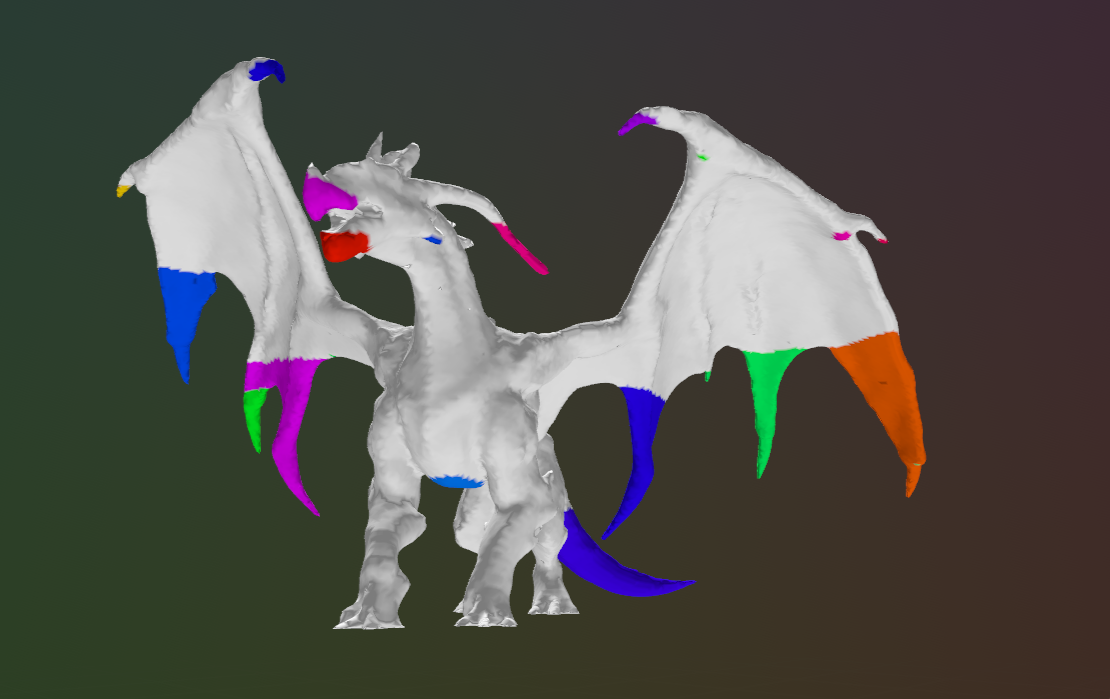
\includegraphics[width=0.5\textwidth]{images/floating_regions_detect.png}
    \caption{Detected floating regions for the test-mesh ``Dragon''}
    \label{fig:floating_regions}
\end{figure}

Efficient detection of floating regions can be achieved using algorithm \cref{alg:float_det}
the idea is that the nodes are sorted from the lowest to the highest, then they are sampled one by one,
and, then visiting the all the nodes reachable form the point, where an arch that go from $A$ to $B$ is 
considered valid only if the layer of $B$ is grater or equal to the layer of $A$.
This ensures that we cannot go ``downward'' when exploring the graph, and therefore that
we cannot explore a floating region unless we start from a point inside that floating region.
While the graph is being explored, we mark nodes that have been visited to avoid visiting the same
node twice, and increasing the time complexity. Once an exploration is completed we can decide if
the explored area is a floating region or not. This can be simply done by checking if the height
of the ``source'' node is equal to zero (or at least is below a certain threshold),
if this is the case we can say that the source was attached to the ground, and therefore
the region is not floating. If this is not the case however, the area we have explored must be a 
floating region. We can also be sure that the nodes we have extracted is the lowest point in the region,
thanks to the sorting we did at the beginning. The sorting also ensures that we start exploring from
the nodes that are close to the ground, avoiding a situation where a floating region is expanded
too much and reach zones that are actually not considered ``floating''.

\begin{algorithm}[h]
\caption{Floating Regions Detection}
\begin{algorithmic}[1]
    \Require $G$ Graph that represent the mesh
    \Ensure $\mathcal{F}$ Set of floating regions 

    \Procedure{ExploreUpward}{$G, s, V$} \Comment{Collect the component reachable going up from $s$}
        \State $R \gets \emptyset$
        \State $Q \gets \{s\}$ \Comment{Initialize the queue with the node}
        \While{$\lnot \Call{IsEmpty}{Q}$} \Comment{repeat untill queue is empty}
            \State $n \gets \Call{Pop}{Q}$
            \State $V(n) \gets true$
            \State $R \gets \Call{Append}{R, n}$
            \For{$a \in \Call{Adjacent}{G, n}$ with } \Comment{Explore adjacent neighbors}
                \If{ $\Call{LayerOf}{a} \geq \Call{LayerOf}{n} \land \lnot V(a)$ } \Comment{Filter by non visited, and $\geq$ layer}
                    \State \Call{Push}{Q, a}
                \EndIf
            \EndFor
        \EndWhile
        \State \Return $R$
    \EndProcedure

    \Statex


    \Procedure{FloatingRegionsDetection}{$G$}
        \State $\mathcal{F} \gets \emptyset, \quad V \gets \emptyset$ \Comment{Detected regions and visited nodes}
        \For{$n \in \Call{SortNodesByHeight}{G}$}
            \If{$V(n)$}
                \State \textbf{continue} \Comment{Already part of a component}
            \EndIf
            \State $R \gets \Call{ExploreUpward}{G, s, V}$ \Comment{Exploring grpah, while only moving ``uppward''}
            \If{$\Call{HeightOf}{s} > 0$} \Comment{If the node is detached from the ground}
                \State $F \gets \Call{AddFloatingRegion}{F, R}$ \Comment{Mark the explored node as a floating region}
            \EndIf
        \EndFor
        \State \Return $\mathcal{F}$
    \EndProcedure
\label{alg:float_det}
\end{algorithmic}
\end{algorithm}



\section{Criticality Grouping}
\label{sec:criticality_grouping}


\section{Contact Points Optimization}
\label{sec:contact_points_opt}


\section{Contact Points Grouping}
\label{sec:contact_points_grouping}


\section{Support Structure Optimization}
\label{sec:sup_struct_opt}

\subsection{Cost Function}
\label{sec:sup_struct_opt_cf}



\section{Exporting}
\label{sec:exporting}
exp



      \chapter{Results}
\label{cha:results}

Now that the inner workings of the algorithm have been explained we will continue with the 
results of the evaluation procedure. The aim here is to understand if the proposed algorithm
is working as intended, and see how it compares against some industry standard solutions.
In order to do so we will first explain our methodologies, then we will take a look at the loss
functions of the optimizer in order to verify that the optimization loop is working as intended.
Afterward we will move to the proper evaluation section where we will compare our solution
with a few industry standard using three key metrics (namely material used, optimization time, and printing
time). Finally we will move show a few real world printing tests to see how well the generated
support actually behaved when printed.

\section{Methodologies}

Before we start with our results we must state the methodologies. Those include the 3D models we used 
to evaluate our solution (the dataset), the ``Baseline Methods'' (i.e. the current industry standard
solution that we will compare our result with), and the Hardware and Software used to run the tests.

\subsection{3D Models}

Evaluating a support generation algorithm require of course the need to have some 3D models to evaluate 
the solution on. Since the research field of optimizing support structure generation for additive manufacturing
is quite niche, there is not a standard dataset that we can simply pick and use. Therefore we have manually
selected three models. We should note that those three models are not representative of the average object
printed by a regular user, this is because most 3D printing models are explicitly designed to be printed without
the need for supports, and would therefore be terrible testcases four our need. For this reasons we have 
explicitly ``charry piked'' models that require an heavy use of supports, so that we could better
appreciate the difference between the various approaches.
The three models we selected are a ``Dragon'' and a ``Candlestick'' taken from the ``printables'' online repository
and ``Armadillo'' taken from Stanford's 3D Scanning Repository.

\subsection{Baseline Methods}

Selecting our baselines methods was a bit challenging as there is no clear ``state of the art''
for what we are trying to do. The two papers that we have looked at in the \ref{cha:prev_literature}
chapter are not concerted with FDM 3D printing, and don't consider the necessary requirements of 
stiffness, making them not really suitable for our application. Furthermore their code is not publicly
available, We have even asked the authors access to the code for comparison use only
but they were unable to fulfill our request due to contractual obligation with industrial partners.
This left only with the options provided by the industry ``Normal'' and ``Tree'' supports (that we have
looked at in the \ref{cha:prev_literature} chapter).

\subsection{Hardware}

All runs have been conducted on an i7 14700HX laptop cpu with 64GB of ram.
The test have been executed while the laptop was fully charged, and connected to the power
plug, without any kind of power saving enabled.
The 3D printer used is an first generation Elegoo Century Carbon 3D printer using
Elegoo PLA as the material of choice.

\subsection{Software}

The test were run on Linux (NixOS 25.11 to be specific) and the code was 
written in Rust, and compiled in release mode without any specific compiler flag.
The rustc version was 1.93.1, and the toolchain used was the stable one.
The code was written to take advantage of multithreading, with the optimization
process regularly saturating all the CPU cores.

\subsection{Tests Number and Naming}

To reduce variability whe have have run our algorithm 5 times for each 
3D model for a total of 15 tests. In the case of the industry standard solutions we
instead only run once, as the variability of those is quite small if not zero.
In the case of the testcase ``Dragon'' we had to manually add some supports after
the one generated by the ``Tree'' algorithm failed to print four times in a row.
For this reason there are two different testcases for the dragon plus tree support combo.
Table \ref{tab:algorithm_maming} show the full list of the tests that have been performed,
with the algorithm and model associated with every test run.


\begin{table}[htbp]
  \centering
  \caption{Testcase list with algorithm and model used}
  \label{tab:algorithm_maming}
  \hspace{4pt}
  \begin{tabular}{lll}
    \toprule
    Test ID & Algorithm & Model \\
    \midrule
    ES1D & Evo Strut (ours) & Dragon \\
    ES2D & Evo Strut (ours) & Dragon \\
    ES3D & Evo Strut (ours) & Dragon \\
    ES4D & Evo Strut (ours) & Dragon \\
    ES5D & Evo Strut (ours) & Dragon \\
    ES1A & Evo Strut (ours) & Armadillo \\
    ES2A & Evo Strut (ours) & Armadillo \\
    ES3A & Evo Strut (ours) & Armadillo \\
    ES4A & Evo Strut (ours) & Armadillo \\
    ES5A & Evo Strut (ours) & Armadillo \\
    ES1C & Evo Strut (ours) & Candlestick \\
    ES2C & Evo Strut (ours) & Candlestick \\
    ES3C & Evo Strut (ours) & Candlestick \\
    ES4C & Evo Strut (ours) & Candlestick \\
    ES5C & Evo Strut (ours) & Candlestick \\
    \midrule
    TSD & Tree Supports & Dragon \\
    CTSD & Custom Tree Supports & Dragon \\
    TSA & Tree Supports & Armadillo \\
    TSC & Tree Supports & Candlestick \\
    \midrule
    NSD & Normal Supports & Dragon \\
    NSA & Normal Supports & Armadillo \\
    NSC & Normal Supports & Candlestick \\
    \bottomrule
  \end{tabular}
\end{table}


\section{Loss Function Trends}

In this section we will print the loss functions, in order to verify that the optimizer
is working properly, however unlike some more traditional optimization problems that have
a single loss function in our case we have many. Infant, as we detailed in chapter \ref{cha:support_opt_alg}
we have separated the optimization problem into three different stages, each of them with it's own
loss function, Furthermore, even within a single stage, we often use the divide and conquer approaches
where instead of solving an single optimization problem we have optimized many smaller one for a more efficient
computation. For example, in the case of the support structure optimization stage for testcase ES1D, the
support problem has been divided into seven different subproblems, and the resulting loss function of each
of the seven run, as well as the total can be seen in figure \ref{fig:individual_problems_loss}.
It should be noted that in the chart the $x$ axis representing the number of iterations has been normalized
in the range 0-1, since every run used a different number of iterations to converge.
We have a total of 45 of this type of graph (5 testcases $\times$ 3 models $\times$ 3 pipeline stages), and
those can be seen in the official github repository, however for in this thesis we decided to only put 
9 aggregates (\ref{fig:es_dragon_cpg} to \ref{fig:es_candlestick_sso}). In this set of aggregates graphs we have grouped
the optimizer run by model and pipeline stage. In every graph we can see the total loss function
of every one of the five runs, plus a single average loss function that gives the idea on how well
the algorithm is optimizing. This means, for example, that the ``Total'' line of graph \ref{fig:individual_problems_loss}
is the transparent blue line in graph \ref{fig:es_dragon_sso}.


\begin{figure}[h]
    \centering
    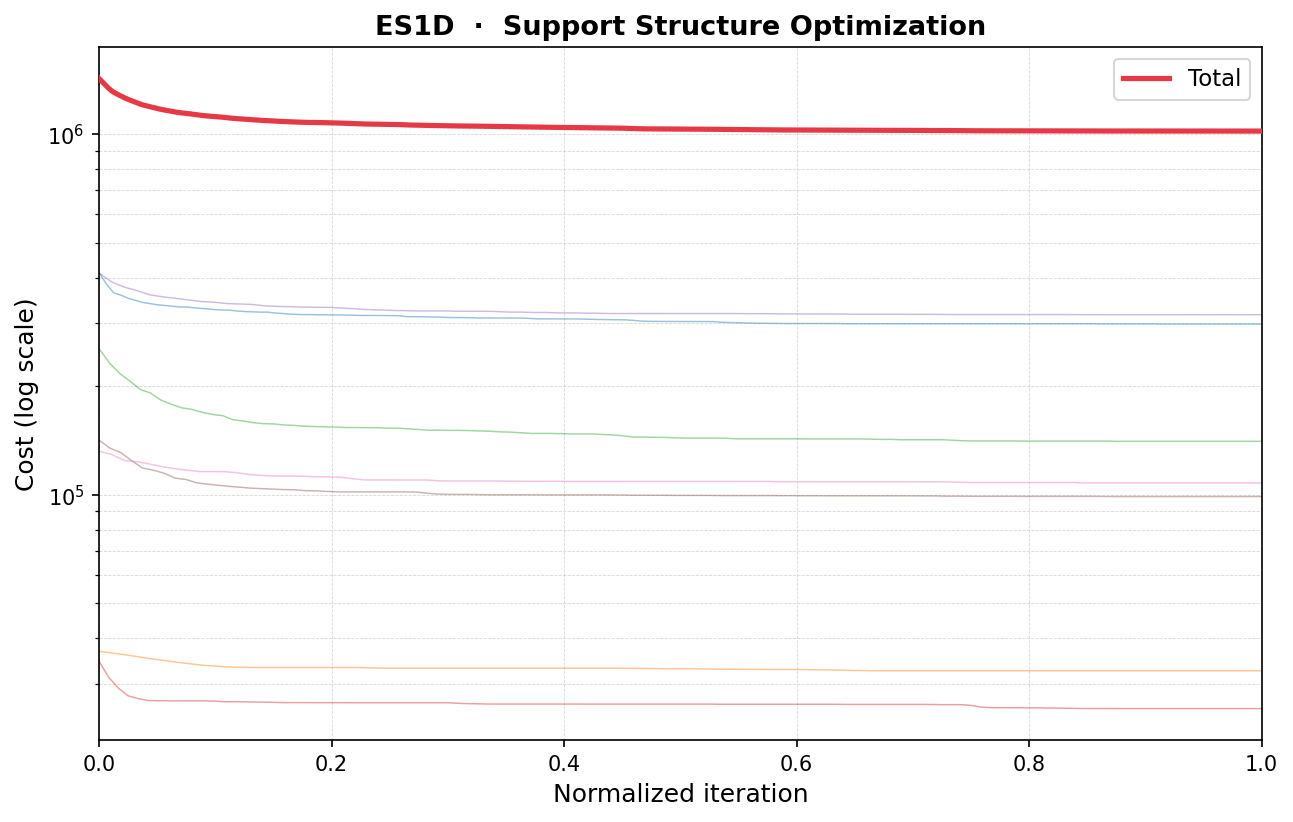
\includegraphics[width=0.5\textwidth]{images/ES1D_support_structure_optimization.png}
    \caption{Loss function of the support structure optimization stage for testcase ES1D}
    \label{fig:individual_problems_loss}
\end{figure}


Looking at all the loss functions we can note how the algorithm is performing quite well (at least
from the point of view of the loss function). 
The first thing that we can note when observing the threads, is that the loss
never degreases, this is of course to be expected given that all three of our optimizers use elitism
in their evolution process. Some of the graph (especially the one about the contact point optimization
stage) are particularly smooth, this both a symptom of the fact that there are a few averages/summations
smoothing out the process, and also of the fact that the first optimization stage is by far the easiest
and more linear of the three.
In some of the graph, we can see that all testcases from one to five at the end converge to a similar value
of the loss function, but on some others (most notably \ref{fig:es_dragon_sso} and \ref{fig:es_candlestick_cpg})
we can see that the different runs converge to different final values
for the loss function. This is almost certainty caused by the optimizer getting stuck in a local minimum
and not being able to further improve the loss, which is a pretty common scenario in most genetic algorithm and gradient
descent like optimizers. If anything our choice to use a three stages optimization problem is increasing
the likelihood of this type of scenario occurring, as every new stage can diverge from the ``optimal'' path
creating a cascade effect that can substantially vary the final output.
However we should not overstate the impact that this effect has on the quality of the solutions, 
even acknowledging that some of the testcases did not perform as well as others the overall thread
is still quite good, with the rate of improve decreasing over time, but still managing a substantial
improvement by the end of the run.



\begin{figure}[H]
    \centering
    \begin{minipage}{0.48\textwidth}
        \centering
        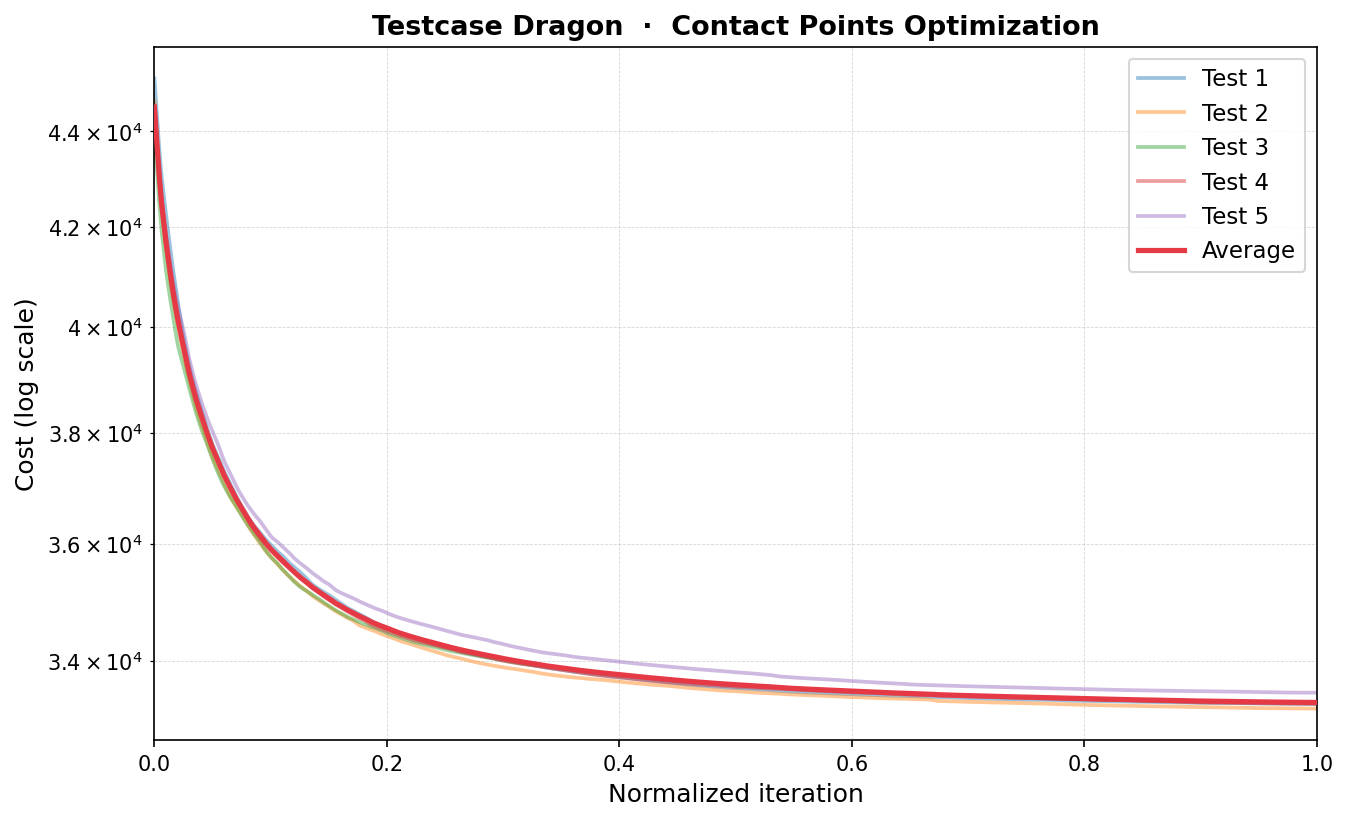
\includegraphics[width=\textwidth]{images/ES_Dragon_contact_points_optimization.png}
        \caption{Contact points optimization loss trend for the Dragon model}
        \label{fig:es_dragon_cpo}
    \end{minipage}
    \hfill
    \begin{minipage}{0.48\textwidth}
        \centering
        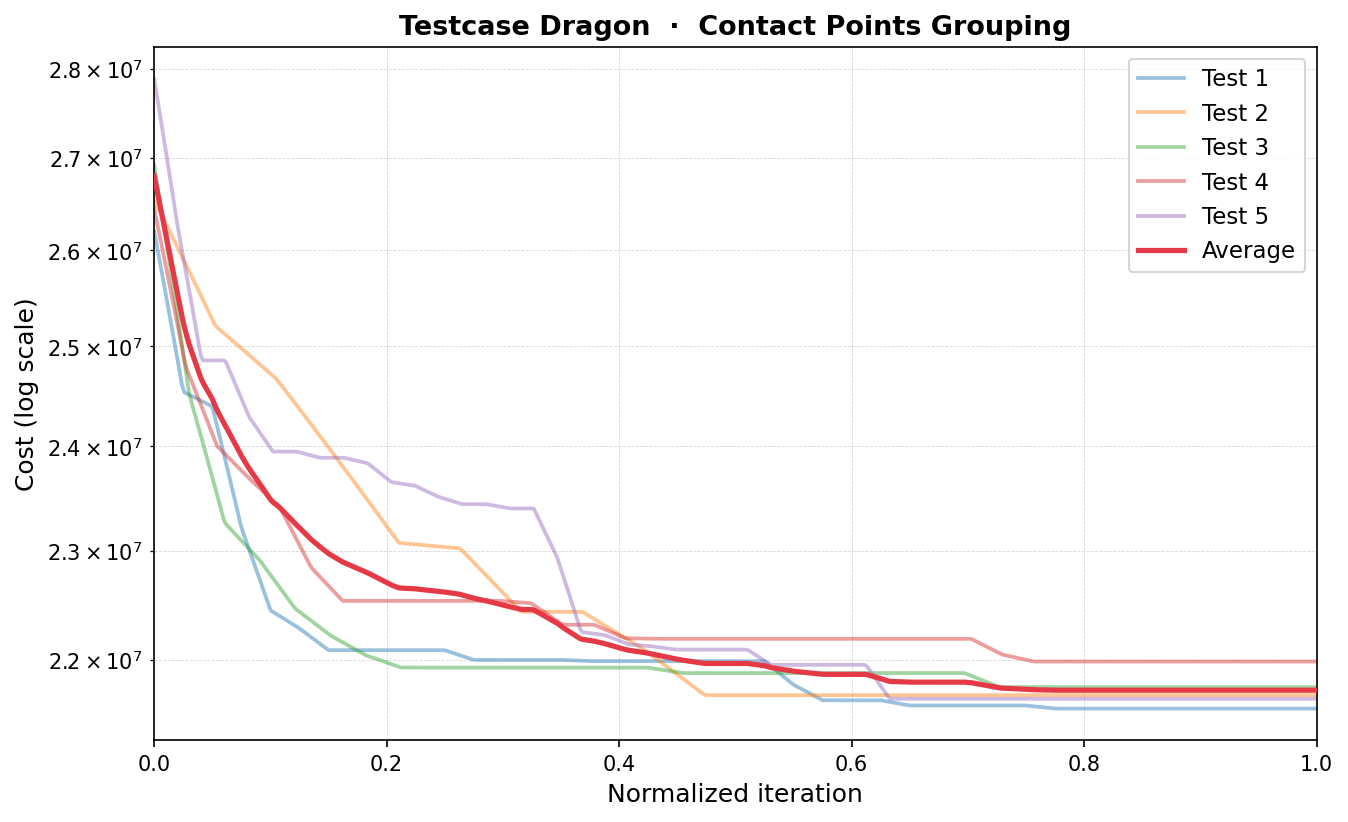
\includegraphics[width=\textwidth]{images/ES_Dragon_contact_points_grouping.png}
        \caption{Contact points grouping loss trend for the Dragon model}
        \label{fig:es_dragon_cpg}
    \end{minipage}
\end{figure}

\begin{figure}[H]
    \centering
    \begin{minipage}{0.48\textwidth}
        \centering
        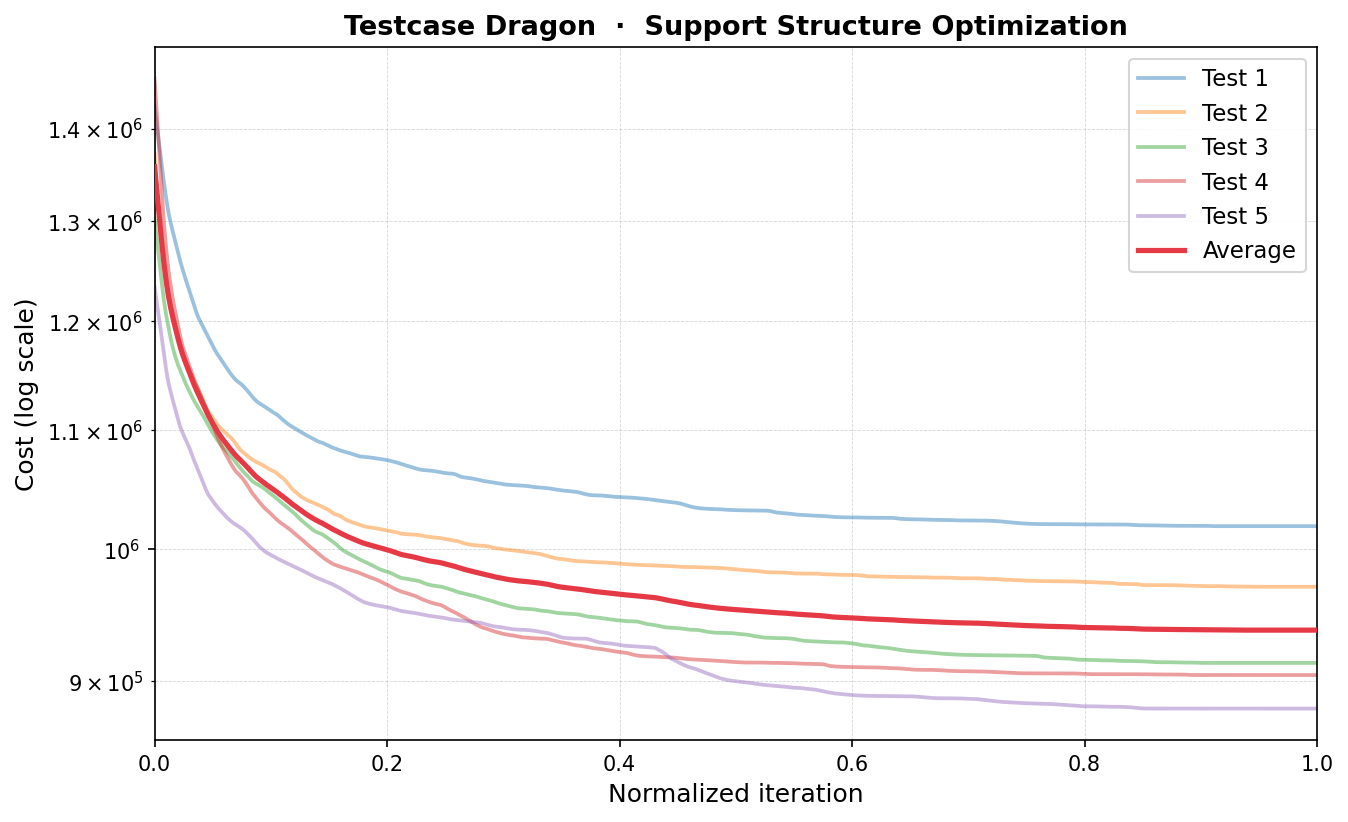
\includegraphics[width=\textwidth]{images/ES_Dragon_support_structure_optimization.png}
        \caption{Support structure optimization loss trend for the Dragon model}
        \label{fig:es_dragon_sso}
    \end{minipage}
    \hfill
    \begin{minipage}{0.48\textwidth}
        \centering
        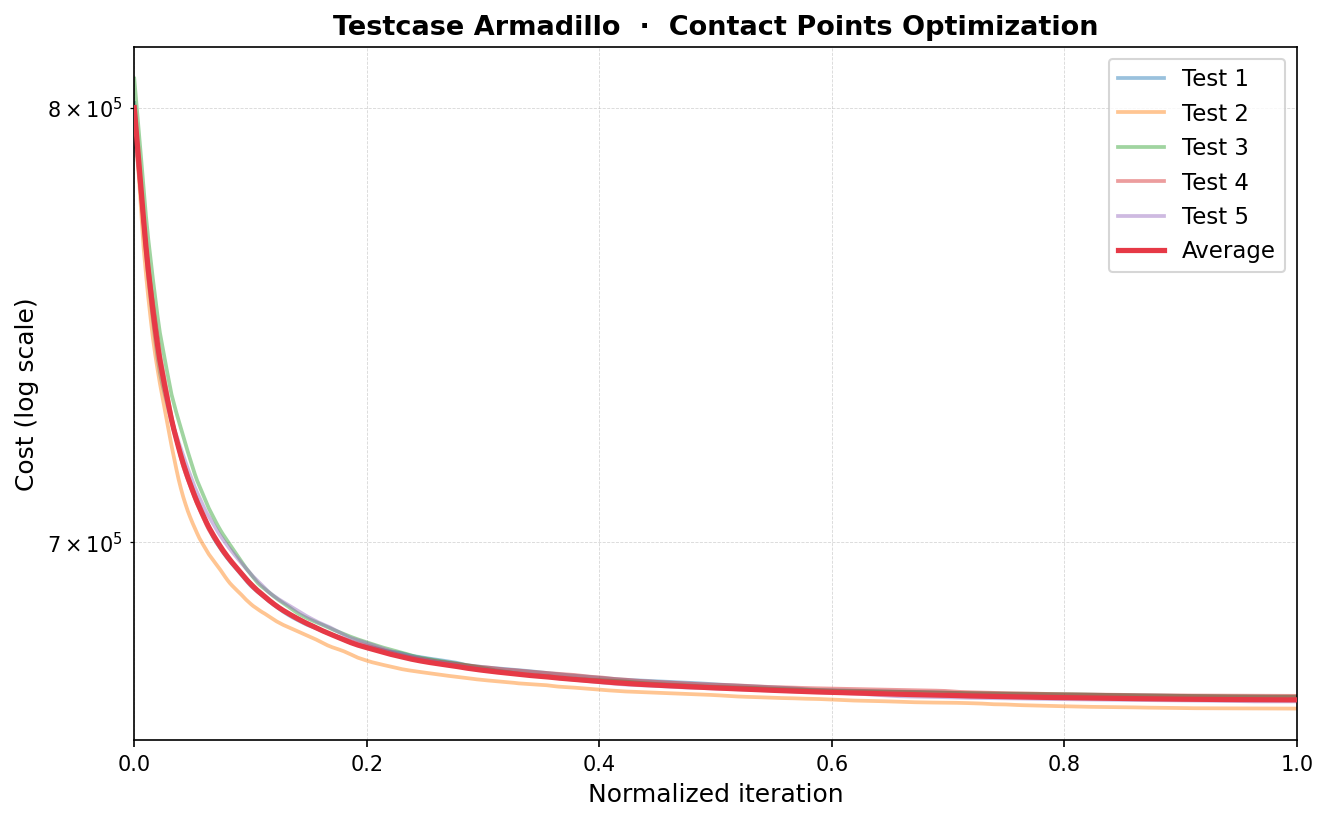
\includegraphics[width=\textwidth]{images/ES_Armadillo_contact_points_optimization.png}
        \caption{Contact points optimization loss trend for the Armadillo model}
        \label{fig:es_armadillo_cpo}
    \end{minipage}
\end{figure}

\begin{figure}[H]
    \centering
    \begin{minipage}{0.48\textwidth}
        \centering
        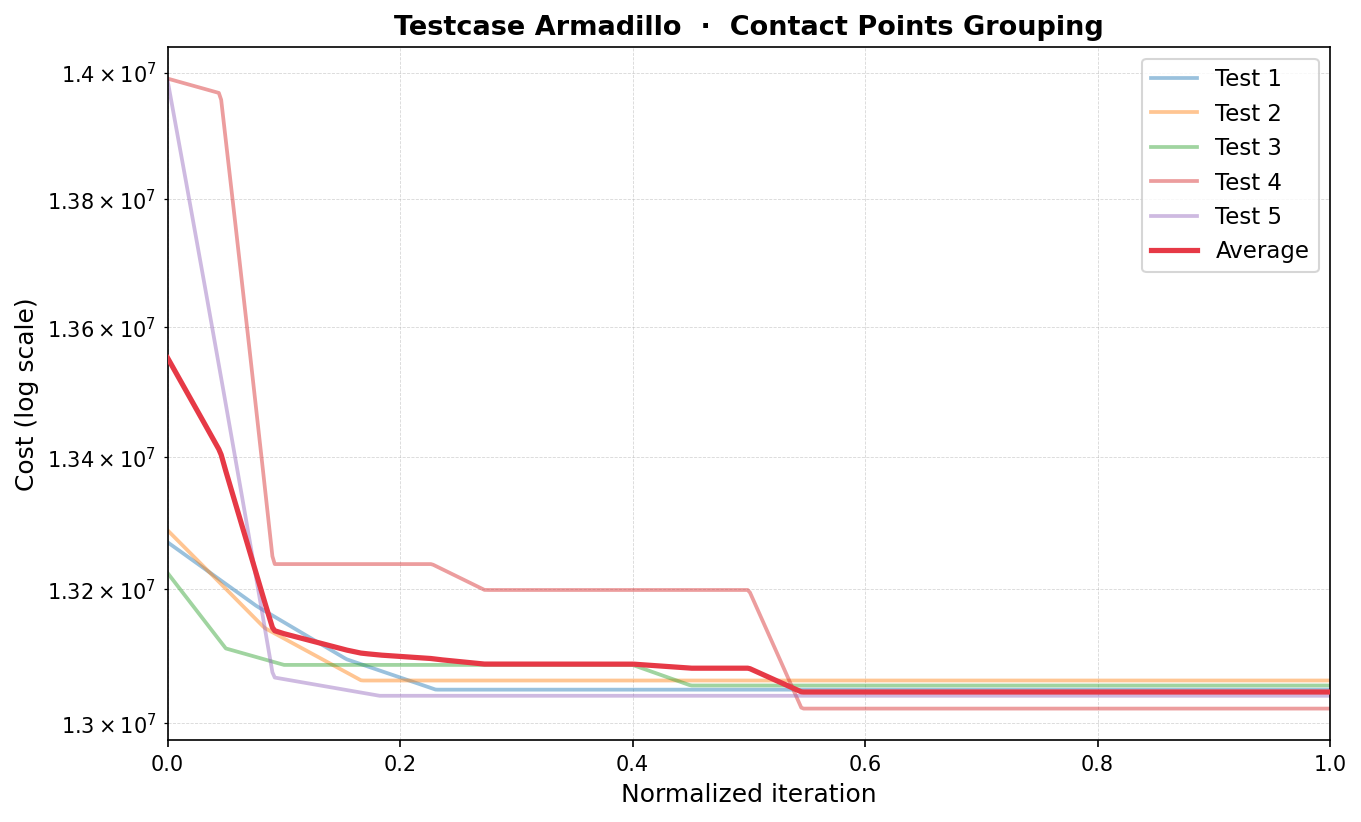
\includegraphics[width=\textwidth]{images/ES_Armadillo_contact_points_grouping.png}
        \caption{Contact points grouping loss trend for the Armadillo model}
        \label{fig:es_armadillo_cpg}
    \end{minipage}
    \hfill
    \begin{minipage}{0.48\textwidth}
        \centering
        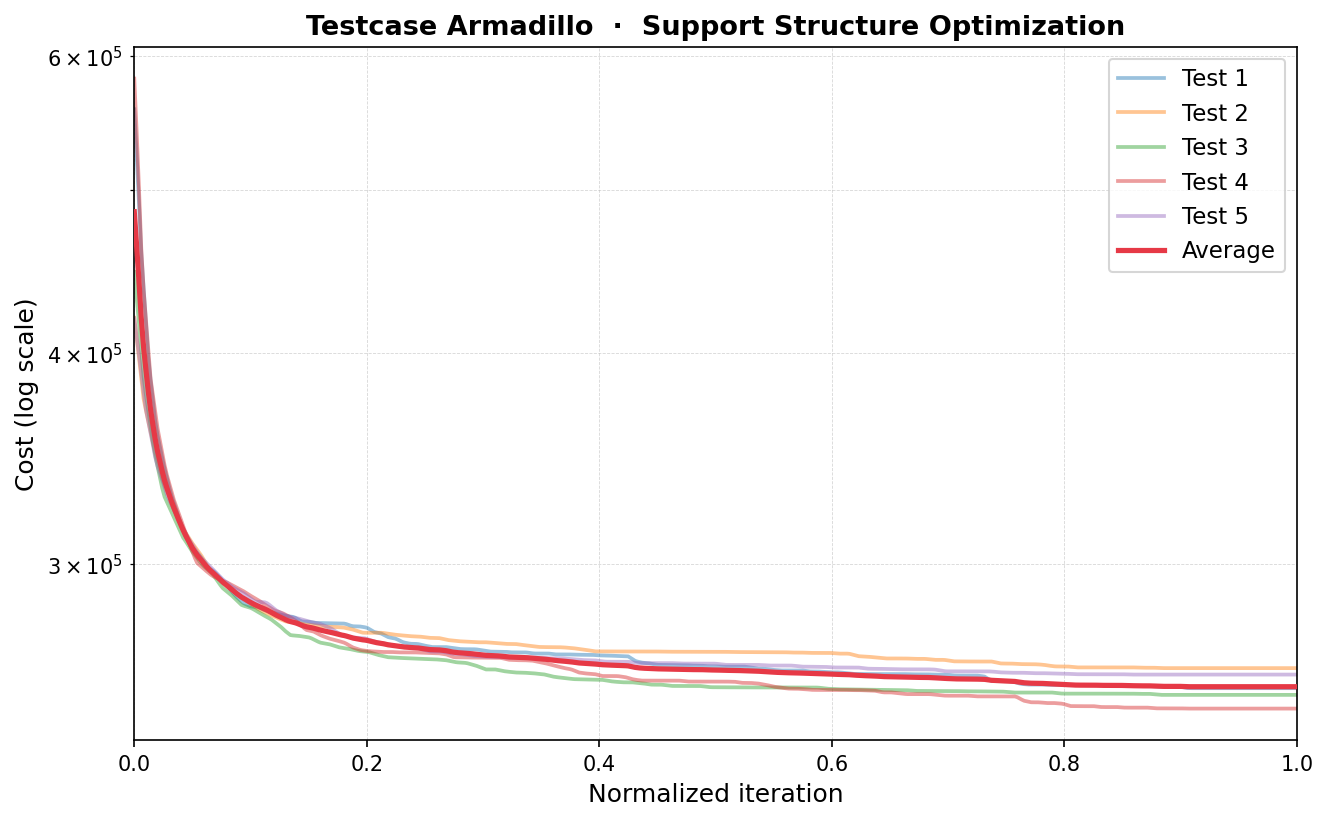
\includegraphics[width=\textwidth]{images/ES_Armadillo_support_structure_optimization.png}
        \caption{Support structure optimization loss trend for the Armadillo model}
        \label{fig:es_armadillo_sso}
    \end{minipage}
\end{figure}

\begin{figure}[H]
    \centering
    \begin{minipage}{0.48\textwidth}
        \centering
        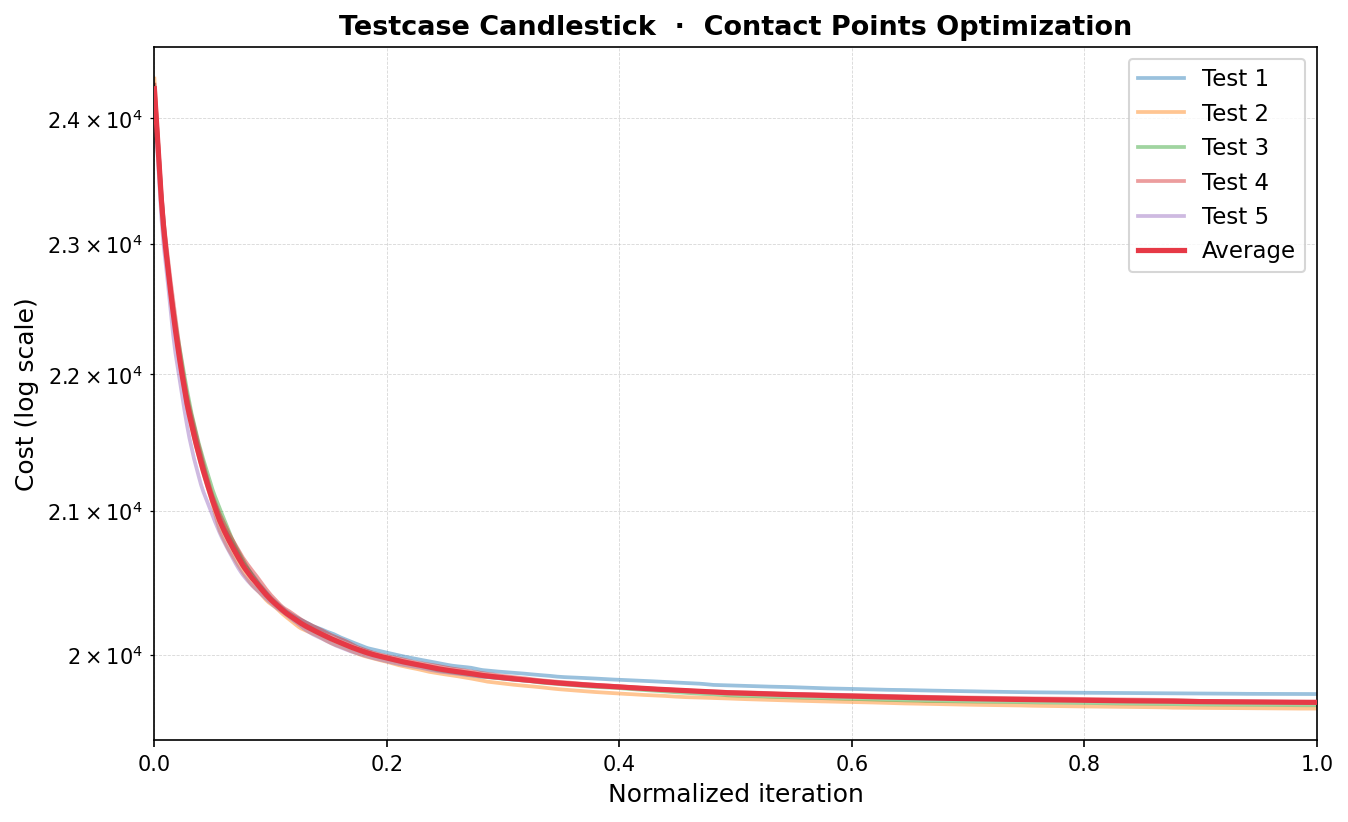
\includegraphics[width=\textwidth]{images/ES_Candlestick_contact_points_optimization.png}
        \caption{Contact points optimization loss trend for the Candlestick model}
        \label{fig:es_candlestick_cpo}
    \end{minipage}
    \hfill
    \begin{minipage}{0.48\textwidth}
        \centering
        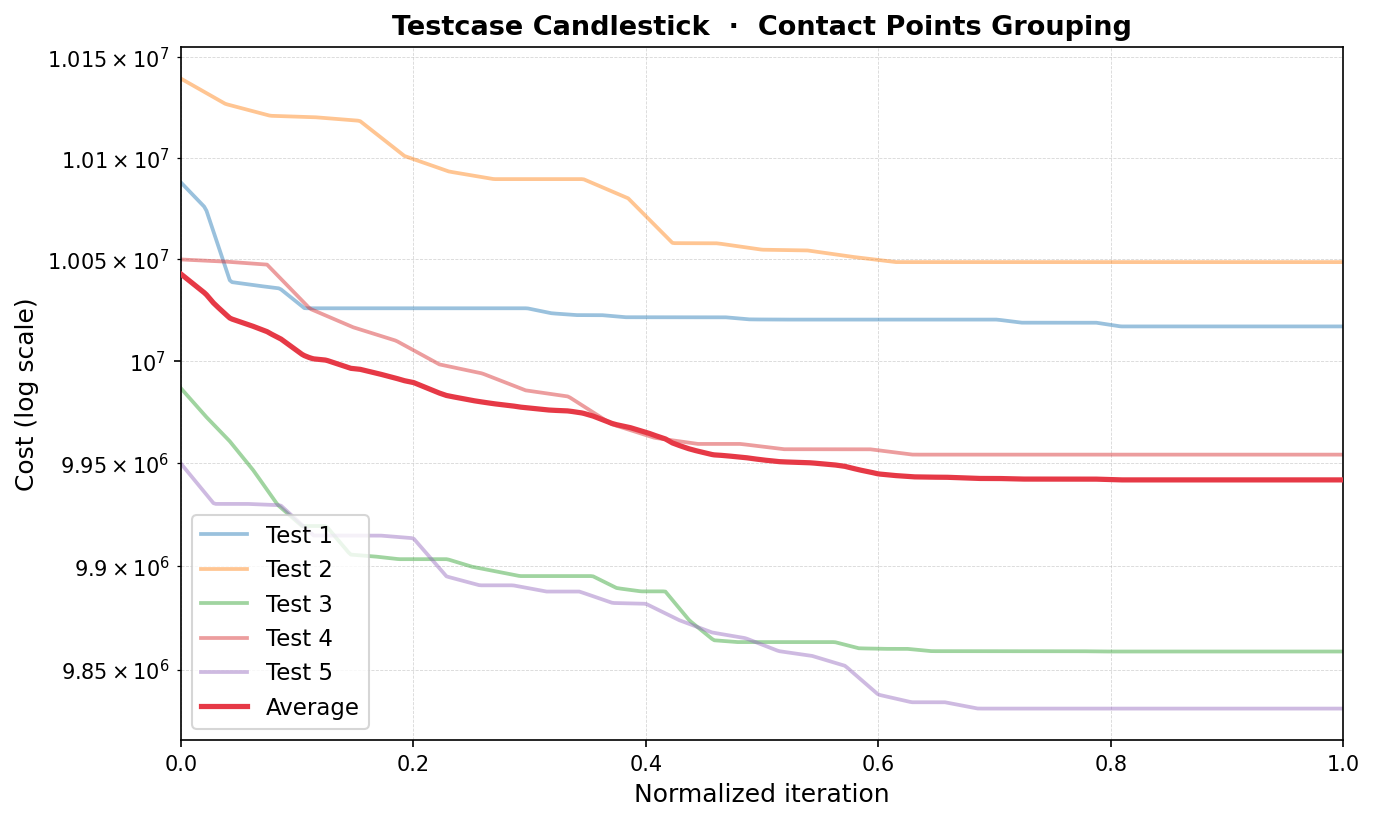
\includegraphics[width=\textwidth]{images/ES_Candlestick_contact_points_grouping.png}
        \caption{Contact points grouping loss trend for the Candlestick model}
        \label{fig:es_candlestick_cpg}
    \end{minipage}
\end{figure}

\begin{figure}[H]
    \centering
    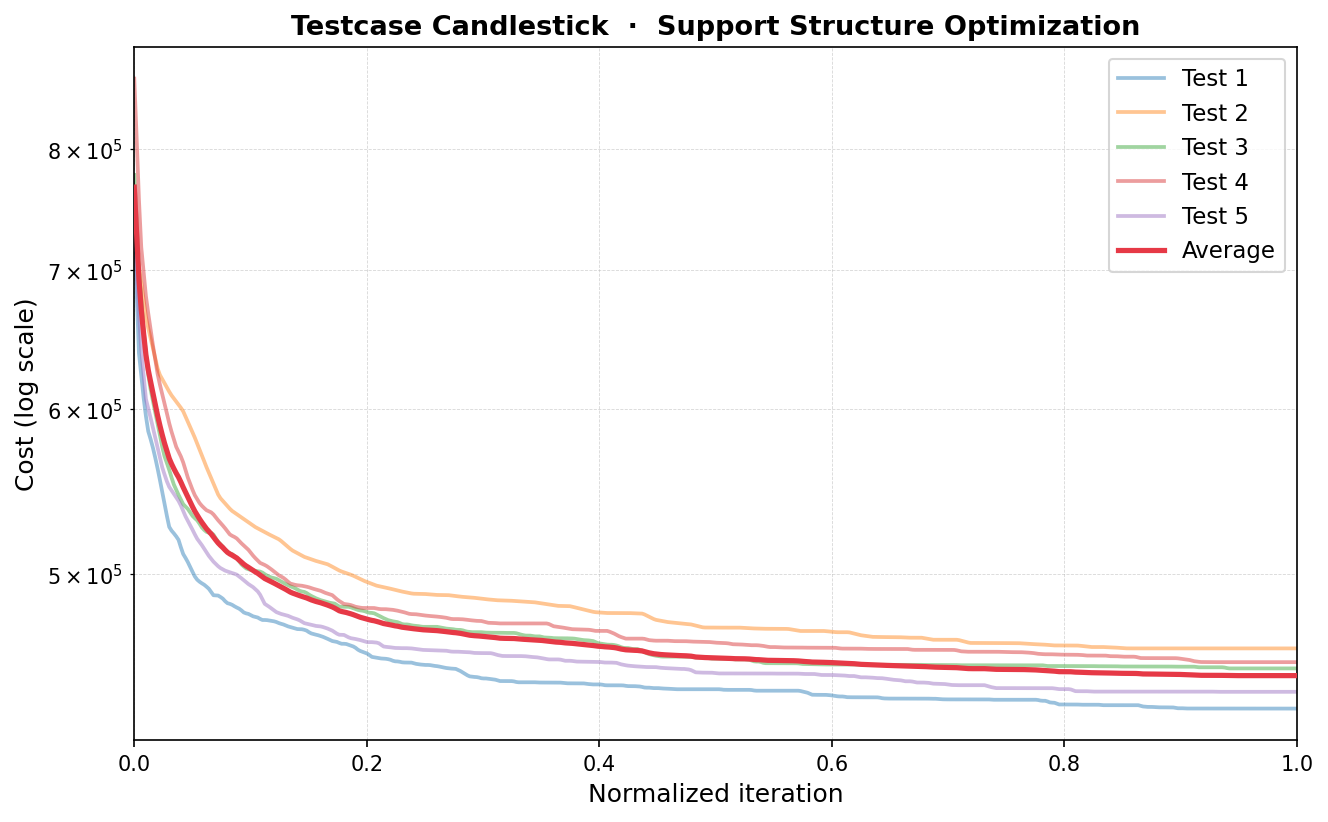
\includegraphics[width=0.5\textwidth]{images/ES_Candlestick_support_structure_optimization.png}
    \caption{Support structure optimization loss trend for the Candlestick model}
    \label{fig:es_candlestick_sso}
\end{figure}

\section{Reduction In material usage}

\section{Execution Time}

\section{Print Time}

\section{Print Tests}


      \chapter{Conclusions}
\label{cha:conclusions}
conc




      

      
    \endgroup


    % bibliography - bibtex format
    %
    % add chapter to index
    \addcontentsline{toc}{chapter}{Bibliography}
    % alphabetical order of authors
    \bibliographystyle{plain}
    \bibliography{biblio}
%%%%%%%%%%%%%%%%%%%%%%%%%%%%%%%%%%%%%%%%%%%%%%%%%%%%%%%%%%%%%%%%%%%%%%%%%%
%%%%%%%%%%%%%%%%%%%%%%%%%%%%%%%%%%%%%%%%%%%%%%%%%%%%%%%%%%%%%%%%%%%%%%%%%%
%% Nota
%%%%%%%%%%%%%%%%%%%%%%%%%%%%%%%%%%%%%%%%%%%%%%%%%%%%%%%%%%%%%%%%%%%%%%%%%%
%% In the bibliography, all the sources consulted for the dissertation 
%% have to be cited and listed in alphabetical order by the 
%% first author's surname.
%%
%% According to the source material, the quotation has to be as follows:
%%
%% BOOKS
%% Surname and initial/s of the name/s of the author/s, date of edition,
%% publishing house and (if applicable) number of edition.
%% 
%% JOURNAL ARTICLES 
%% Surname and initial/s of the first name/s of the author/s,
%% title of the article, name of the journal, volume number, issue number
%% and page numbers.
%% 
%% CONFERENCE PAPERS
%% Surname and initial/s of the name/s of the author/s,
%% year of the conference, title of the article, name of the conference,
%% place of the conference, conference dates, page numbers.
%% 
%% CITING WEB RESOURCES
%% The consulted webpages have to be listed in alphabetical order. 
%% It is necessary to:
%%   - Copy the specific URL (the web address) of the consulted webpage
%%   - If available, indicate the surname and first name of the author/s,
%%     the title and subtitle of the text
%%   - If available, indicate the last date you retrieved the webpage
%%     (day/month/year).   
%%%%%%%%%%%%%%%%%%%%%%%%%%%%%%%%%%%%%%%%%%%%%%%%%%%%%%%%%%%%%%%%%%%%%%%%%%
%%%%%%%%%%%%%%%%%%%%%%%%%%%%%%%%%%%%%%%%%%%%%%%%%%%%%%%%%%%%%%%%%%%%%%%%%%
    

    \titleformat{\chapter}
        {\normalfont\Huge\bfseries}{Appendix \thechapter}{1em}{}
    % Appendix / attachment section - optional
    \appendix
    \chapter{Title first appendix}

foo


\section{Title}

foo

\subsection{Sub-title}

foo


\chapter{Title first appendix}

foo

\section{Title}

foo

\subsection{Sub-title}
foo




\end{document}
